\documentclass[sigconf, pbalance]{acmart}

\acmConference[PRI Project]{Information Processing and Retrieval (PRI) — M.EIC 2025/26}{December 2025}{FEUP, University of Porto}

% --- Packages ---
\usepackage{minted}
\usepackage{xcolor}
\usepackage{adjustbox}
\usepackage{tabularx}
\usepackage{makecell}
\usepackage{booktabs}
\usepackage{float}
\usepackage{hyperref}
\graphicspath{{images/}}

% --- Minted code style ---
\definecolor{bg}{HTML}{F8F8F8}
\setminted{
    bgcolor=bg,
    frame=single,
    framesep=2mm,
    fontsize=\scriptsize,
    baselinestretch=1.05,
    breaklines=true,
    breakanywhere=true,
    breaksymbolleft={},
    breaksymbolright={},
    linenos=true,
    numbersep=5pt,
    autogobble=true
}

\author{Lu\'is Fiunte}
\email{up202208819@up.pt}
\affiliation{%
  \institution{FEUP, Universidade do Porto}
  \city{Porto}
  \country{Portugal}
}

\author{Marta Cruz}
\email{up202205028@up.pt}
\affiliation{%
  \institution{FEUP, Universidade do Porto}
  \city{Porto}
  \country{Portugal}
}

\author{Ricardo Ramos}
\email{up202206349@up.pt}
\affiliation{%
  \institution{FEUP, Universidade do Porto}
  \city{Porto}
  \country{Portugal}
}

% --- Document ---
\begin{document}

\title[Enhancing Pharmaceutical Discovery: A Hybrid Information Retrieval System for Drug Labels]{%
  Enhancing Pharmaceutical Discovery: A Hybrid Information Retrieval System for Drug Labels
}

\begin{abstract}
  This report presents the design and implementation of a comprehensive pharmaceutical information retrieval system. The project follows a structured development pipeline, beginning with the ingestion and cleaning of the OpenFDA drug label dataset to establish a reliable domain-specific corpus. Building on this foundation, we developed a search engine using Apache Solr, evaluating various indexing strategies and field-based relevance models. To overcome the limitations of keyword-based retrieval, we implemented a hybrid search architecture that combines sparse BM25 signals with dense vector representations from PubMedBERT, optimizing the fusion via Reciprocal Rank Fusion (RRF). The system is accessible through a modern web interface featuring smart query rewriting, result clustering, and real-time visualization of chemical structures. This work demonstrates the effective integration of traditional information retrieval techniques with state-of-the-art neural models to enhance discovery in the biomedical domain.
\end{abstract}

\begin{CCSXML}
  <ccs2012>
  <concept>
  <concept_id>10002951.10003317</concept_id>
  <concept_desc>Information systems~Information retrieval</concept_desc>
  <concept_significance>500</concept_significance>
  </concept>
  </ccs2012>
\end{CCSXML}

\ccsdesc[500]{Information systems~Information retrieval}

\keywords{Information Retrieval, OpenFDA, Drug Label Dataset, Solr}

\maketitle

% =============================
% Part 1: Data Preparation
% =============================


\section{Introduction}
Drug labeling data represents one of the most information-rich and complex resources in the pharmaceutical field~\cite{fang2016druglabel,nature_fdalabel}. Each label contains structured metadata such as product identifiers and manufacturing details, as well as long unstructured text describing therapeutic use, dosage, active ingredients, and safety warnings~\cite{nature_fdalabel,fda_fdalabel}. These records are critical for both healthcare professionals and automated systems that require reliable access to regulatory information~\cite{fang2016druglabel,fda_fdalabel}.

The dataset analyzed in this work was created using the OpenFDA API, a public data service provided by the U.S. Food and Drug Administration (FDA)~\cite{openfdaapi,acm_openfda}. This API grants access to thousands of official drug label submissions, which were programmatically extracted and combined into a single, cleaned dataset~\cite{openfdaapi,fda_fdalabel,frontiers_extraction}. Each entry represents a specific drug or drug product, identified by unique codes such as \texttt{product\_ndc}, \texttt{package\_ndc}, and \texttt{set\_id}. The dataset also includes descriptors such as \texttt{therapeutic\_category} and \texttt{brand\_name}, along with free-text fields like \texttt{indications\allowbreak\_and\allowbreak\_usage}, \texttt{dosage\allowbreak\_and\allowbreak\_administration}, and \texttt{warnings}~\cite{frontiers_extraction,liu_dli}.


After extraction, the data were standardized to ensure consistency and to handle incomplete or missing fields~\cite{liu_dli,nature_fdalabel}. The resulting collection retains both structured and unstructured information, making it a valuable foundation for building information retrieval systems in later phases~\cite{fang2016druglabel,nature_fdalabel}.


\section{Data Source Authority and Quality}
The OpenFDA platform is an official initiative maintained by the U.S. Food and Drug Administration, designed to provide open access to regulatory and safety data. Each record within the \textit{drug label} endpoint originates directly from approved submissions or post-marketing updates.

This source offers several advantages in terms of reliability:

\begin{itemize}
  \item \textbf{Authority:} The FDA is the primary regulatory agency for pharmaceutical products in the United States, ensuring data authenticity.
  \item \textbf{Traceability:} Each label is linked to official identifiers (e.g., \verb|set_id|, \verb|product_ndc|), enabling cross-referencing with other FDA datasets.
  \item \textbf{Data Integrity:} The OpenFDA API enforces standardized JSON schemas and field structures, minimizing format inconsistencies.
\end{itemize}

Beyond its internal consistency, the OpenFDA platform is widely regarded as a foundational reference for pharmaceutical information. Data derived from FDA sources are routinely integrated into commercial pharmacy databases (e.g., First Databank, Lexicomp, and Micromedex), used by major electronic health record (EHR) systems, and cited in regulatory and academic research.

\textit{As of November 2024, the FDALabel database contains over \textbf{158,000} human drug labeling documents—including \textbf{97,289} OTC and \textbf{57,699} prescription labels—providing comprehensive pharmaceutical coverage for operational and analytical applications. The dataset is available at:} \underline{\textit{\url{https://nctr-crs.fda.gov/fdalabel/ui/search}}}.



\section{Exploratory Data Analysis}
Exploratory Data Analysis (EDA) was performed to understand the characteristics of the dataset, detect inconsistencies, and guide the cleaning process. The original records were retrieved in \texttt{JSON} format via the OpenFDA API and subsequently converted into a unified \texttt{CSV} file using the data extraction pipeline described in Annex~A. This CSV format facilitated the application of cleaning routines, exploratory and retrieval-oriented analysis, and index construction. Beyond descriptive statistics, a retrieval-oriented analysis was conducted to evaluate which textual attributes contribute most to the construction of a search index.


\subsection{Therapeutic Categories}
Figure~\ref{fig:categories} shows the distribution of therapeutic categories. Each drug entry may belong to multiple categories, all of which were counted individually. The most frequent categories include \textit{analgesics}, \textit{NSAIDs}, and \textit{antibiotics}. These distributions indicate high thematic diversity, which will be essential for coverage evaluation in retrieval experiments.

\begin{figure}[htbp]
  \centering
  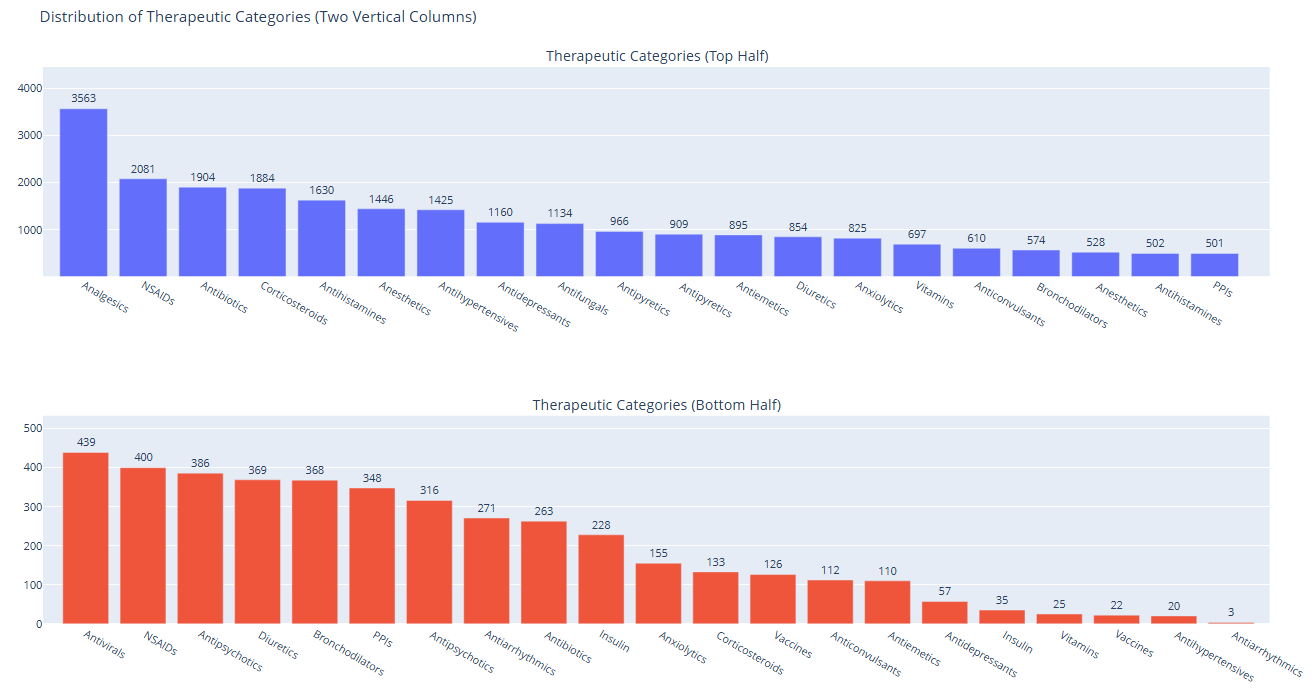
\includegraphics[width=0.40\textwidth]{categories.png}
  \Description{Bar chart showing the frequency of different therapeutic categories such as analgesics, NSAIDs, and antibiotics.}
  \caption{Distribution of therapeutic categories in the dataset.}
  \label{fig:categories}
\end{figure}

\subsection{Key Descriptive Fields and Search-Oriented Statistics}
Table~\ref{tab:text-eda} summarizes the main textual fields in the dataset: \newline \texttt{indications\_and\_usage}, \texttt{dosage\allowbreak\_and\allowbreak\_administration}, \texttt{purpose}, \texttt{warnings}, and \texttt{active\allowbreak\_ingredients}. These represent the unstructured portion of the drug label documents and contain the richest information for search and retrieval tasks.

Metrics such as average word count, vocabulary size, and type-token ratio were computed to assess text richness and variability. The \texttt{indications\_and\_usage} field showed the highest textual volume, frequently spanning several hundred words with detailed therapeutic descriptions and clinical terminology. The \texttt{warnings} section displayed similar complexity, dominated by regulatory and safety-related language.

In contrast, \texttt{purpose} and \texttt{active\_ingredients} are concise and structured, usually limited to a few keywords or chemical names. These fields are particularly useful for faceted or field-specific searches. The \texttt{dosage\_and\_administration} field falls in between—long enough for meaningful keyword analysis but structured enough for section-based retrieval.

Overall, this variability in verbosity and vocabulary density reflects the heterogeneous nature of the dataset. From an IR perspective, this is advantageous: longer sections enrich ranking through contextual relevance, while concise fields improve precision via targeted filtering. These insights guided the selection and weighting of indexable fields in later project stages.

\begin{table}[htbp]
  \centering
  \caption{Summary of main textual fields relevant for retrieval.}
  \begin{tabular}{|l|c|c|c|c|}
    \hline
    \textbf{Field} &
    \makecell{\textbf{Average}                   \\ \textbf{Word Count}} &
    \makecell{\textbf{Standard}                  \\ \textbf{Error}} &
    \makecell{\textbf{Max}                       \\ \textbf{Words}} &
    \makecell{\textbf{Unique}                    \\ \textbf{Words}} \\
    \hline
    \makecell{Indications                        \\ And Usage}      & 162.2 & 1.33 & 1994  & 17795 \\
    \hline
    \makecell{Dosage and                         \\ Administration}  & 477.9 & 3.97 & 8307  & 30948 \\
    \hline
    Purpose        & 7.3   & 0.15 & 604  & 4967  \\
    \hline
    Warnings       & 430.1 & 5.06 & 5229 & 16940 \\
    \hline
    \makecell{Active                             \\ Ingredients}         & 13.5  & 0.16 & 415   & 5801  \\
    \hline
    \makecell{Inactive                           \\ Ingredients}       & 26.1  & 0.26 & 1349  & 8186  \\
    \hline
  \end{tabular}
  \label{tab:text-eda}
\end{table}

\subsection{Routes of Administration}
Figure~\ref{fig:route} shows the distribution of administration routes. The most common are \textit{oral}, \textit{topical}, and \textit{intravenous}. This attribute will later serve as a facet field for refining search results.

\begin{figure}[htbp]
  \centering
  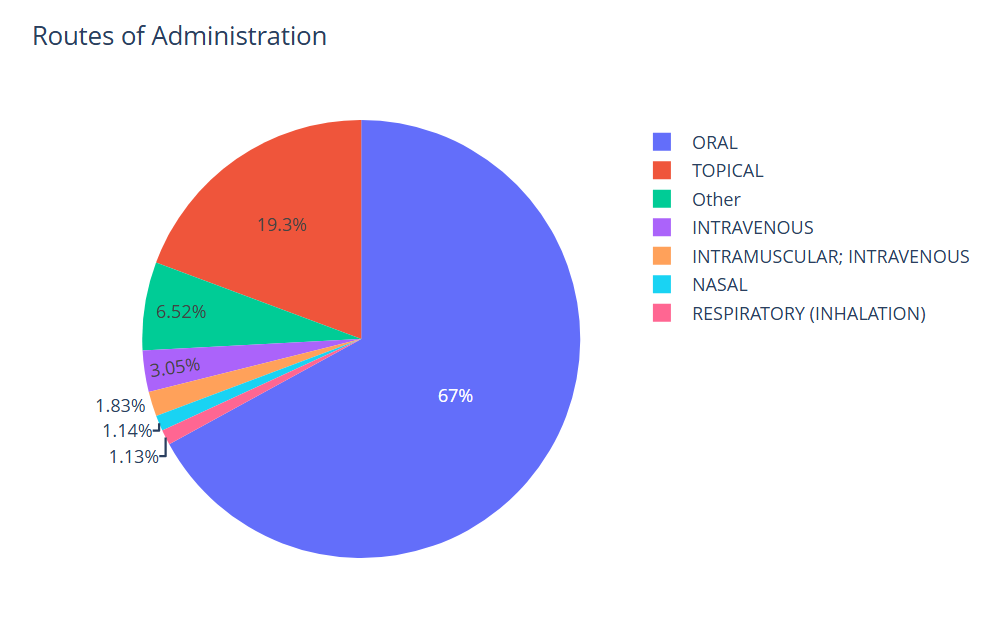
\includegraphics[width=0.40\textwidth]{route.png}
  \Description{Bar chart displaying the distribution of administration routes, with oral being the most frequent, followed by topical and intravenous.}
  \caption{Distribution of administration routes.}
  \label{fig:route}
\end{figure}

\section{Script Implementation for Database Construction}
A Python-based pipeline automates extraction, processing, and storage of drug label information from the OpenFDA API.

\begin{enumerate}
  \item \textbf{Category and Term Management:} A dictionary of therapeutic categories with associated keywords guides API queries.
  \item \textbf{API Interaction:} Iterative retrieval with pagination and rate-limit management.
  \item \textbf{Data Extraction:} Standardization of field names and flattening of nested structures.
  \item \textbf{Database Construction:} Merging entries by identifier, resolving duplicates, and preserving multi-category records.
  \item \textbf{Output Generation:} Export of the cleaned dataset to CSV for reproducibility.
  \item \textbf{Error Handling:} Automatic retries and exception logging ensure robustness.
\end{enumerate}

\begin{figure}[htbp]        % usa [htbp] se não quiseres forçar aqui
  \centering
  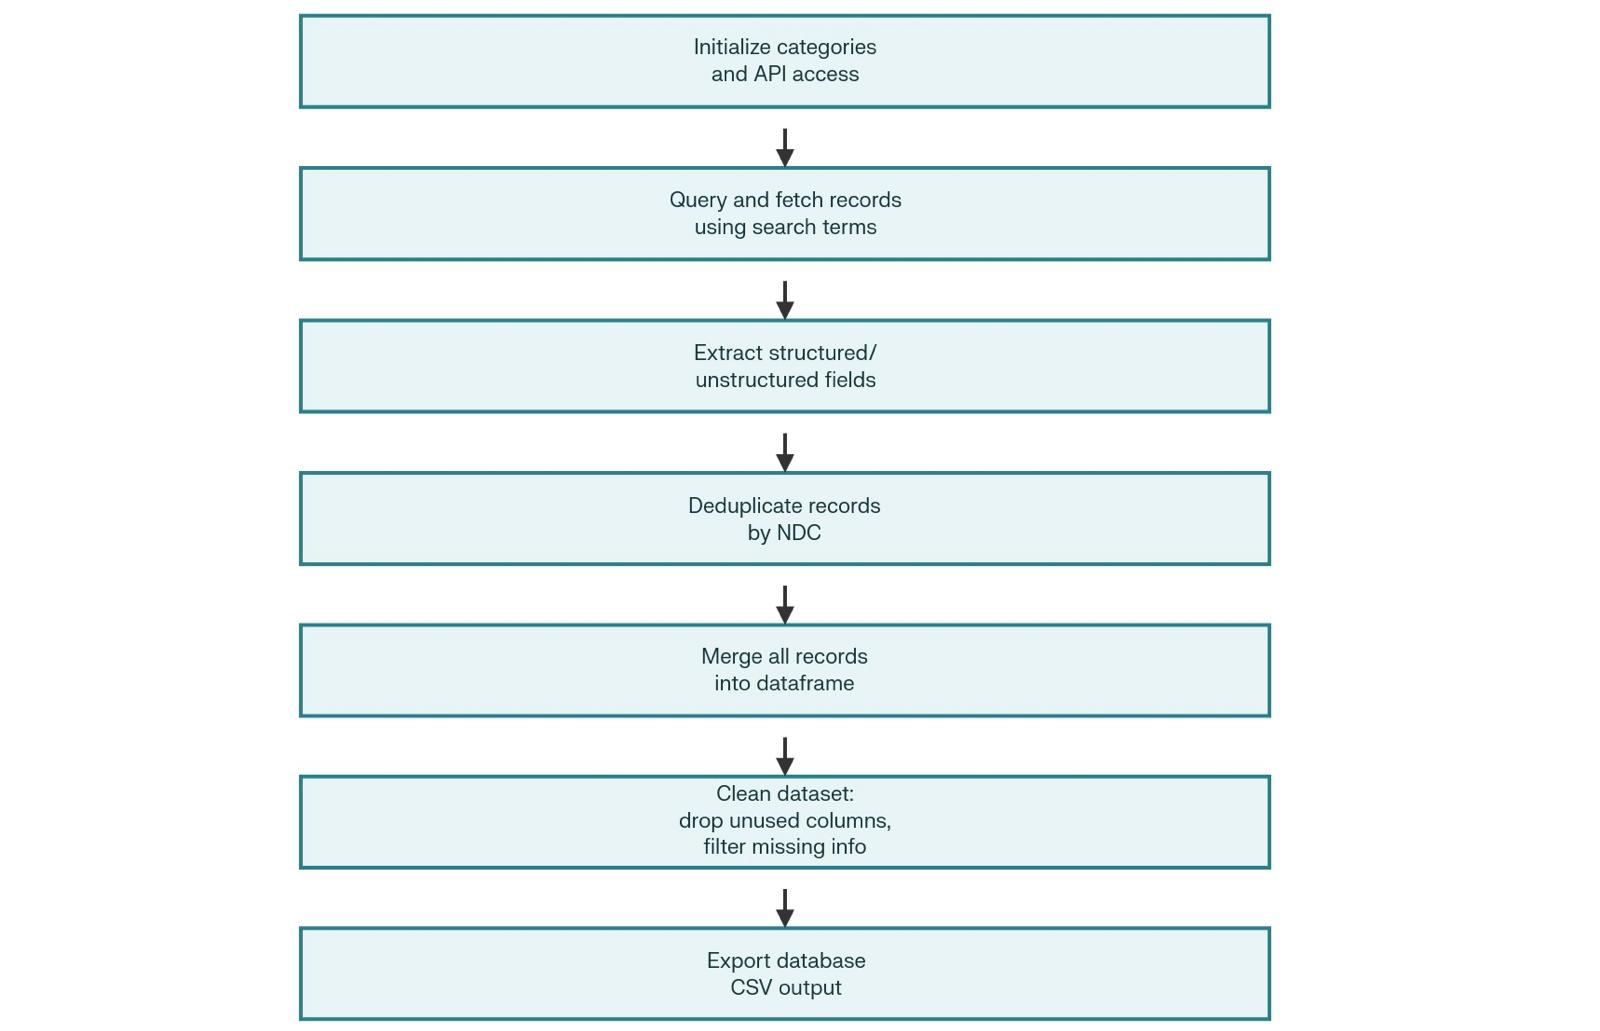
\includegraphics[width=0.85\linewidth]{Pipeline.jpeg}
  \Description{Flowchart illustrating the data cleaning pipeline: API Category Management to API Interaction, Data Extraction, Database Construction (Merge/Resolve), Output Generation (CSV), and Error Handling.}
  \caption{Pipeline}
  \label{fig:pipeline}
\end{figure}

\section{Data Cleaning and Handling of Incomplete Entries}

The raw dataset obtained from the OpenFDA API was highly unstructured and contained a substantial number of incomplete entries. Many fields were sparsely populated; for example, over 85\% of entries lacked a UPC code, approximately 70\% were missing storage and handling information, and around 67\% did not include purpose. Even core identifiers and naming fields, such as brand name, generic name, and manufacturer, were missing in more than 55\% of the records.

To improve the dataset's reliability and usability, several steps were taken:

\begin{enumerate}
  \item \textbf{Dropping irrelevant attributes:} Columns not essential for the analysis or search tasks were removed to streamline the dataset. The UPC was discarded because more relevant identifiers, such as primary and product NDCs, were already present for every entry. The search term column was removed as it primarily served as a helper attribute during dataset development and does not contribute to downstream analysis or search functionality.


  \item \textbf{Removing entries without key identifiers:} All records that lacked any of the essential identification fields --- \textit{brand name, generic name, product type, package NDC, or manufacturer} --- were removed. Entries missing these values provided virtually no identifying information, making them unusable for reliable analysis or classification. Notably, every entry missing one of these identifiers was also missing all of them. This pattern reaffirms the authenticity and consistency of the source data, as the absence of identifiers reflects a genuine lack of information for those products rather than a data quality issue in the dataset itself.



  \item \textbf{Assigning therapeutic categories:} Each drug entry was tagged with a therapeutic category representing a general type of medicine. This facilitated grouping and analysis without adding extensive detail, and also provides a structured layer of classification that will be useful when implementing the search engine, which is the core of the project.
\end{enumerate}

After cleaning, all retained entries had valid names, and missing values in key identifiers dropped to 0\%. Core descriptive fields—such as substance name, UNII, route, indications and usage, and dosage and administration—were nearly complete, with fewer than 2\% of missing values. The \texttt{purpose} field remained partially incomplete (58\%), as it is optional and often omitted for generic drugs. This limitation is minor, since the \texttt{indications\_and\_usage} field already provides the clinically relevant information needed for search and retrieval tasks in Solr.

This cleaning process ensured that the final dataset, is more structured, reliable, and suitable for downstream analysis and search indexing, while retaining high coverage of core identifying and categorical information.

\section{Key Attributes for Search Engine Implementation}
The cleaned dataset includes 22 attributes combining structured metadata and rich unstructured text. The following are the most relevant for building a Solr-based search system:

\begin{itemize}
  \item \textbf{indications\_and\_usage:} Core field describing therapeutic purpose; high textual variability, essential for relevance ranking.
  \item \textbf{dosage\_and\_administration:} Describes recommended dosages and forms; suitable for detailed phrase and proximity search.
  \item \textbf{purpose:} Concise description of intended drug use; valuable for quick retrieval and query expansion.
  \item \textbf{warnings:} Rich in safety-related terms; critical for semantic matching and alert-based filtering.
  \item \textbf{active\_ingredients:} Supports fielded search and fil\-tering by compound name.
  \item \textbf{inactive\_ingredients:} Useful for chemical comparison and allergy-related searches.
  \item \textbf{route} and \textbf{therapeutic\_category:} Structured facets enabling advanced filtering.
  \item \textbf{manufacturer\_name:} Useful for metadata queries and result grouping.
\end{itemize}

For implementation, textual fields will be tokenized using a domain-adapted analyzer (standard + bio\-medical stopword removal), while structured fields will be stored as filterable facets. This setup supports hybrid ranking based on both full-text similarity and field weighting.

\section{Conceptual Model}
Each record in the dataset represents a \textbf{drug label document}, combining structured identifiers and unstructured descriptions. Conceptually, the entities are:

\begin{itemize}
  \item \textbf{Drug Product:} Core entity, identified by NDC codes.
  \item \textbf{Label Document:} Textual and regulatory information per drug.
  \item \textbf{Active Ingredient:} Linked to multiple products.
  \item \textbf{Manufacturer:} Produces multiple drug products.
  \item \textbf{Therapeutic Category:} Groups drugs by pharmacological class.
\end{itemize}

In this project, each record represents a single drug label document and all relevant attributes—structured identifiers, textual fields, and categorizations—are combined in one table. Since the schema is flat, with every field stored together under 'DrugLabel' and no linked tables or relationships, a standard UML diagram was not required for the initial phase. All conceptual entities discussed (drug product, label, ingredient, manufacturer, category) are just attributes in the same record, not modeled separately.

\section{Information Needs and Follow-up Directions}
The dataset supports several information retrieval scenarios:

\begin{itemize}
  \item \textbf{Condition-based Retrieval:} Find drugs by disease or symptom (e.g., ``treatments for hypertension'').
  \item \textbf{Safety Queries:} Retrieve all drugs containing specific warnings or contraindications.
  \item \textbf{Ingredient-based Lookup:} Identify products containing a given compound.
  \item \textbf{Comparative Retrieval:} Compare dosage or safety profiles across similar drugs.
  \item \textbf{Manufacturer-based Search:} Retrieve all drugs from a specific producer.
  \item \textbf{Trend Analysis for Therapeutic Categories:} Search for trends in drug products and active ingredients associated with a specific health problem or therapeutic category. For example, ``what active ingredients are most commonly used in medications for diabetes'' or ``how has the choice of therapeutic class changed for hypertension drugs in recent years''.
\end{itemize}

\subsection{Characterization of Follow-up Information Needs}
In future work, these information needs will guide the design and evaluation of IR experiments using the dataset. Planned directions include:

\begin{itemize}
  \item \textbf{Retrieval Evaluation:} Measuring precision and recall for category-based and ingredient-based queries, using different Solr configurations.
  \item \textbf{System Enhancement:}  Exploring methods for semantic query expansion (e.g., synonym-based retrieval), advanced ranking with word embeddings, and user-oriented faceted exploration.
\end{itemize}


% (End of Part 1)



% =============================
% Part 2: Information Retrieval
% =============================
\section{Solr Indexing Configuration}

Following the data preparation, the drug label dataset was converted into a collection suitable for Solr indexing. This phase focused on configuring the schema to support the specific information needs identified in the previous section, ensuring that both structured metadata and unstructured text fields were indexed appropriately for efficient search and accurate retrieval.

\subsection{Indexing Process}

To ensure a strictly reproducible environment, the project infrastructure is defined using Docker Compose. The setup consists of a primary Solr container (based on the official \texttt{solr:9} image) and a transient setup container that automates configuration.

In order to simplify working with Docker, a \texttt{Makefile} was created, responsible for orchestrating development workflows and abstracting complex commands into simple, repeatable tasks.

The indexing process followed these steps:

\begin{enumerate}
    \item Ensure the Solr core is available by polling the Solr ping endpoint until a successful response is received. This guarantees that subsequent schema modifications and data uploads will succeed without errors.

    \item Configure the analysis components (tokenizers and filters) by posting \texttt{analysis.json} to the Solr schema API. The analysis setup, including the modification of the \texttt{text\_general} field type to include a \texttt{PorterStemFilterFactory} for stemming, is detailed in Appendix~\ref{appendix:analysis}.

    \item Define the schema fields by posting \texttt{fields.json} to the schema API, specifying field types, storage, indexing, and multi-valued settings. This prevents Solr from automatically inferring types. Details of the add-field requests are provided in Section~\ref{appendix:addfield}.

    \item Set up copy fields by posting \texttt{copy\_fields.json} to the schema API, creating a consolidated \texttt{text\_all} field to enable searching across multiple \texttt{text\_general} fields. The copy-field definitions are provided in Appendix~\ref{appendix:copyfields}.

    \item Add the initial dataset by posting \texttt{data.json} to the Solr update endpoint with \texttt{commit=true}, ensuring that all documents are indexed immediately and are searchable. No annex is needed for the dataset itself.

\end{enumerate}


This automation allows the entire system to be provisioned and indexed using the single \texttt{Makefile}.

\subsection{Indexing Fields and Schema}

The schema design was driven by the specific retrieval requirements of the domain. Fields were categorized and typed as follows:

\begin{itemize}
    \item \textbf{Exact Match Fields (String):} Identifiers like \texttt{productNdc}, \texttt{packageNdc}, and \texttt{setId} were indexed as \textbf{string}. This decision ensures that these fields are not tokenized, preserving their exact alphanumeric structure which is critical for precise looking up, sorting, and faceting. Analyzing these as text would break them into unusable tokens.
    \item \textbf{Full-Text Fields (Text\_general):} Descriptive fields such as \texttt{indicationsAndUsage}, \texttt{warnings}, and \texttt{activeIngredients} contain natural language. They were indexed as \textbf{text\_general}, using a standard tokenizer and a Porter Stemmer. This configuration allows for case-insensitive matching and handles morphological variations (e.g., retrieving "addiction" for "addictive"), which is essential for recall in medical text search.
    \item \textbf{Numeric and Date Fields:} \texttt{version} (\textbf{pint}) and \texttt{effectiveTime} (\textbf{pdate}) were strongly typed to enable range queries (e.g., finding drugs updated in the last year) and mathematical operations in function queries.
\end{itemize}

A unified copy-field, \texttt{text\_all}, was created to aggregate content from all major textual fields. This allows for broad "catch-all" queries without needing to specify every individual field, significantly simplifying the default search behavior. The final schema manually defines 23 fields to prevent Solr's "schemaless" mode from inferring incorrect types (e.g., treating an ID as a number), ensuring index stability.


\section{Query Design and Retrieval Strategy}

In this section, we explore the query strategies employed to retrieve relevant information from the structured medicine dataset. Rather than simple keyword matching, we utilized advanced Solr features to address specific challenges in medical information retrieval.

\subsection{Boosting Strategies}
Relevance scoring was fine-tuned using three types of boosting:

\begin{itemize}
    \item \textbf{Field Boosts (qf):} We assigned higher importance to concise, defining fields. for example, setting \texttt{qf=brand\_name\^{}3 generic\_name\^{}2} ensures that matches in the drug name contribute more to the score than matches in long descriptive text like \texttt{indications\_and\_usage}.
    \item \textbf{Term Boosts (\textasciicircum{}):} Critical query terms were manually boosted to reflect medical priority. For instance, in a query like \texttt{fever\^{}2 headache pregnancy\^{}3}, the term "pregnancy" is weighted heavily to ensure safety-critical constraints are respected in the ranking.
    \item \textbf{Independent Boosts (bf):} To prioritize newer information without strictly filtering out older records, we applied a Reciprocal Rank function on the \texttt{effective\_time} field. This function, \texttt{recip(ms(NOW,effective\_time)...)}, additively boosts recent documents, ensuring that users see the most up-to-date labels first.
\end{itemize}

\subsection{Handling User Input and Precision}
To handle the variability of user input and ensure high precision, we implemented:

\begin{itemize}
    \item \textbf{Fuzzy and Wildcard Search:} Medical terms are often misspelled. We utilized fuzzy search (e.g., \texttt{generic\_name:Ibuprof\textasciitilde{}1}) to match "Ibuprofen" even with typos, and wildcards (e.g., \texttt{addict*}) to capture variations like "addiction" or "addictive".
    \item \textbf{Proximity Search (pf, ps):} We used Phrase Fields (\texttt{pf}) and Phrase Slop (\texttt{ps}) to boost documents where query terms appear close together. For example, finding "ibuprofen" and "allergy" within 5 words of each other in the \texttt{warnings} field is a strong signal of relevance compared to them appearing in unrelated sections of a long document.
\end{itemize}


\subsection{Example Retrieval Setup and Evaluation Criteria}
\label{sec:example-setup}

This section provides a complete demonstration query for a specific, safety-critical information need.

\textbf{Problem / Search Goal:} Suppose we are a pregnant woman experiencing a fever and a headache. The objective is to find an oral-route OTC drug that is medically considered the safest option for use during pregnancy and has been approved or updated recently (2023–2025). The goal is to return results that are relevant, safe, and complete.

\textbf{Example Solr Query:}

\begin{minted}{bash}
q=(fever^4 headache^3)
defType=edismax

qf=purpose^4.0 warnings^3.0 text_all
fq=product_type:("OTC")
fq=route:ORAL
fq=effective_time:[2022-01-01T00:00:00Z TO NOW]

bq=warnings:"safe for pregnancy"~5^3.0
pf=warnings^2.0
\end{minted}

\textbf{Explanation of Logic and Safety Fixes:}
\begin{itemize}
    \item \textbf{q}: Focuses strictly on the user's symptoms ($\texttt{fever}$, $\texttt{headache}$) with specific boosts ($\texttt{\^{}4}, \texttt{\^{}3}$) to ensure the retrieved documents explicitly address the ailment rather than just mentioning the words in passing.
    \item \textbf{fq}: Narrows the result set to documents that meet \textbf{strict usability criteria}: $\texttt{OTC}$ availability and $\texttt{ORAL}$ route. Crucially, it filters for recency using $\texttt{effective\_time}$, removing outdated medical information.
    \item \textbf{qf}: Searches across fields but prioritizes $\texttt{purpose}$ (what the drug is for) and $\texttt{warnings}$ (safety info) over generic text ($\texttt{text\_all}$).
    \item \textbf{bq}: Utilizes a proximity boost ($\texttt{\~{}5}$) to increase the ranking of documents that contain the phrase "safe for pregnancy" (or similar variations where words are within 5 tokens of each other), directly addressing the safety requirement.
    \item \textbf{pf}: Adds a phrase boost to the $\texttt{warnings}$ field to ensure symptom keywords appearing close together in safety sections are ranked higher.
\end{itemize}

\textbf{Manual Evaluation Criteria:}
To achieve a Relevant score (1), the document must satisfy all constraints defined in the project's relevance logic:

\begin{itemize}
    \item \textbf{Symptom Match:} Explicitly indicates treatment for $\texttt{fever}$ or $\texttt{headache}$.
    \item \textbf{Route \& Type:} Specifies an $\texttt{oral}$ administration route (e.g., tablet, liquid) and is classified as $\texttt{OTC}$.
    \item \textbf{Recency:} Includes a product information date within the $\texttt{2023–2025}$ range (evaluated against the $\texttt{effective\_time}$ filter).
    \item \textbf{Safety Profile:} Does \textbf{not} strictly contraindicate use during pregnancy. Note: Standard regulatory warnings such as "consult a health professional before use" are accepted as Relevant (1).
\end{itemize}

Bad results (Irrelevant, Score 0) are those that treat different symptoms, require non-oral administration (e.g., topical, nasal), require a prescription, are outdated, or explicitly forbid use during pregnancy.

\section{Evaluation}
In this section, we evaluate the effectiveness of two distinct retrieval setups as a formal scientific experiment. The objective is to quantitatively measure the retrieval effectiveness of a naive baseline versus our advanced ranking logic mentioned in the previous section, using a manually created "ground truth" for the required safety-critical information need.

\subsection{Evaluation Methodology}

Our methodology follows the standard Information Retrieval (IR) evaluation paradigm, focusing on the single, safety-critical information need regarding pregnancy.

\subsubsection{Information Need}
We define the specific need used for evaluation in Table~\ref{tab:infoneed}.

\begin{table}[h!]
    \centering
    \caption{Information Need and Search Parameters}
    \label{tab:infoneed}
    \begin{tabular}{p{3.0cm} p{4.5cm}}
        \hline
        \textbf{User Scenario}     & A pregnant woman with a fever and headache needs a safe, recent, oral OTC drug.                                                \\
        \hline
        \textbf{Baseline Query}    & \texttt{fever headache pregnancy oral OTC}                                                                                     \\
        \textbf{Advanced Criteria} & \textbf{Must match:} \texttt{product\_type:OTC} AND \texttt{route:\allowbreak ORAL} AND \texttt{effective\_time:[2022 TO NOW]} \\
        \hline
    \end{tabular}
\end{table}

\subsubsection{Retrieval Setups}
We compare the two defined setups:
\begin{itemize}
    \item \textbf{Setup 1 (Baseline):} Serves as a naive control. It queries the text using a simple "bag-of-words" approach (\texttt{q="fever headache pregnancy oral OTC"}) against a generic catch-all field (\texttt{qf=text\_all\^{}1}). Crucially, it \textit{does not} use strict schema filters, relying on keyword matching for terms like "OTC" and "oral".
    \item \textbf{Setup 2 (Advanced):} Uses sophisticated query logic including:
          \begin{itemize}
              \item \textbf{Strict Filtering (\texttt{fq}):} Enforces route:ORAL
                    and product\_type:OTC to remove irrelevant formats immediately.
              \item \textbf{Field Boosting (\texttt{qf}):} Prioritizes core metadata (\texttt{purpose\^{}4, warnings\^{}3}) over generic text.
              \item \textbf{Relevance Boosting (\texttt{bq}):} Boosts documents containing safety phrases (e.g., warnings:\allowbreak "safe for pregnancy"\~{}5\^{}3.0).
          \end{itemize}
\end{itemize}

\subsubsection{Manual Evaluation Process}
A relevance judgment file (qrels.txt) was created using the \textbf{pooling method} (top $K=20$ results from both setups). Each unique document was \textbf{manually evaluated} (with AI-based verification) using a binary relevance scale (1=Relevant, 0=Irrelevant). A document was marked Relevant only if it met all safety criteria: treating the symptoms, being strictly OTC and Oral, and having no pregnancy contraindications.

\subsection{Results and Analysis for Q1}
We executed both queries against our Solr instance and used the \texttt{pytrec\_eval} tool to calculate P@10 (Precision at 10) and AP (Average Precision).

\subsubsection{Comparative Metrics}
Table~\ref{tab:q1results} shows the performance of both systems.

\begin{table}[h!]
    \centering
    \caption{Comparative Metrics for Query Q1}
    \label{tab:q1results}
    \begin{tabular}{l c c c}
        \hline
        \textbf{Metric}    & \textbf{Setup 1 (Base.)} & \textbf{Setup 2 (Adv.)} & \textbf{\% Imprv.} \\
        \hline
        \textbf{AP (Q1)}   & 0.0357                   & 0.5731                  & +1505.3\%          \\
        \textbf{P@10 (Q1)} & 0.1000                   & 0.5000                  & +400.0\%           \\
        \hline
    \end{tabular}
\end{table}

The results indicate a massive disparity in performance. The Advanced setup (Setup 2) achieved an \texttt{Average Precision (AP)}of 0.5731, compared to the negligible 0.0357 of the Baseline. This represents an improvement of over \texttt{1500\%}. Similarly, \texttt{P@10} jumped from 0.1 (1 relevant doc in top 10) to 0.5 (5 relevant docs in top 10), a \texttt{400\% increase}.

\subsubsection{Precision-Recall Curve}
To visualize the performance trade-off, we generated the Interpolated Precision-Recall curve.

\begin{figure}[h!]
    \centering
    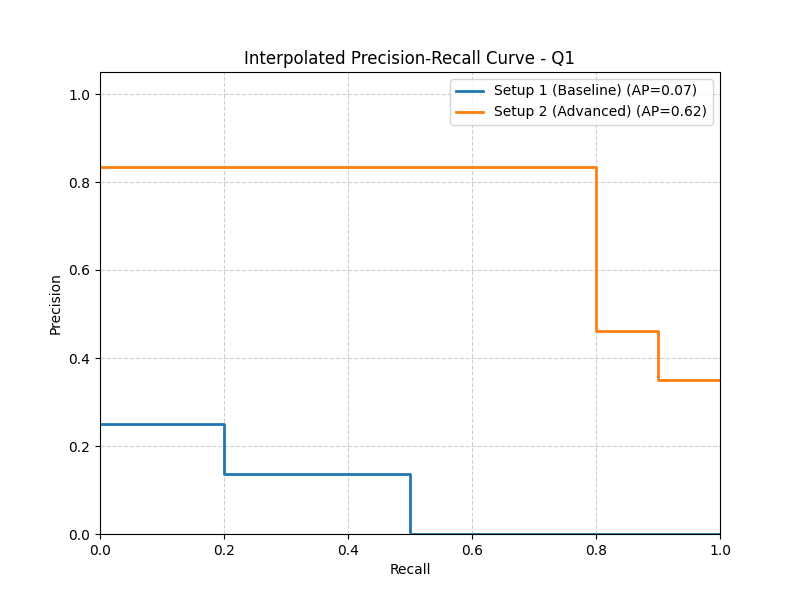
\includegraphics[width=\columnwidth]{pr_curve.png}
    \Description{Interpolated Precision-Recall Curve showing the Advanced Setup (blue line) significantly outperforming the Baseline Setup (orange line). The Advanced line stays high across recall levels, while Baseline drops quickly.}
    \caption{Interpolated Precision-Recall Curve}
    \label{fig:prcurve}
\end{figure}

\subsection{Precision-Recall Analysis}

Figure \ref{fig:prcurve} confirms the dominance of the Advanced setup (Setup 2). Its curve maintains high precision and extends to high recall, demonstrating that the strict filters (\texttt{fq=route:ORAL}) and boosting logic successfully retrieved the majority of safe drugs. The "step-like" shape reflects the distinct relevant documents found.

In contrast, the Baseline curve (Setup 1) is severely truncated, terminating at very low recall. This visual "shortness" indicates a critical \textbf{Recall Failure}: the system missed the majority of relevant documents. The naive keyword search was overwhelmed by noise (e.g., matching "not for oral use"), burying the correct results deep in the ranking where they were not retrieved.

\subsection{Discussion of Results}

The evaluation clearly demonstrates the superiority of the Advanced setup (Setup 2) over the Baseline (Setup 1), with AP increasing from 0.03 to 0.57.

\paragraph{Analysis of Baseline Failure}
The Baseline's poor performance ($P@10 = 0.1$) highlights the limitations of naive "bag-of-words" search in safety-critical domains. By searching for "OTC" and "oral" merely as keywords in the unstructured \texttt{text\_all} field, Setup 1 retrieved numerous irrelevant documents. These included labels where "oral" appeared in negated contexts (e.g., "not for oral use") or where OTC was mentioned only in reference to other products. The lack of structural filtering meant the system could not distinguish between substantial matches (e.g., product form) and incidental text occurrences.

\paragraph{Success of Filter-Boost Strategy}
Setup 2 succeeded because it effectively combined \textbf{hard constraints} with \textbf{soft relevance signals}.
\begin{itemize}
    \item The use of strict filters (\texttt{fq=route:ORAL}) guaranteed that 100\% of the candidate pool was at least administratively correct, eliminating the noise that plagued the baseline.
    \item The proximity boost (\texttt{bq=... "safe for pregnancy"\^{}3}) acted as a semantic proxy, successfully pushing documents that explicitly addressed safety to the top.
\end{itemize}

\paragraph{Limitations}
Despite the strong performance, the current setup relies on exact metadata coverage. Drugs with missing `route` or `effective\_time` fields would be excluded regardless of their text content. Additionally, the boolean text match for "safe for pregnancy" is rigid; a semantic search approach using embeddings (planned for future work) would robustly handle variations like "safe for expectant mothers" that the current keyword-based system might miss.


\clearpage
% (End of Content)


% =============================
% Part 3: Interface and advanced features
% =============================
\section{Hybrid Search Model Development}
\label{sec:hybrid-search-best-model}

This section details the methodology for determining the optimal hybrid search configuration for our pharmaceutical document retrieval system. The approach is divided into two distinct phases, as illustrated in Figure~\ref{fig:hybrid-search-methodology}:

\begin{enumerate}
    \item \textbf{Best Dense Vector Model Selection}: Evaluating multiple state-of-the-art embedding models using Approximate Nearest Neighbor (ANN) search to identify the most effective dense vector representation.
    \item \textbf{Optimal Hybrid Weight Tuning}: For the selected dense model, determining the optimal $\alpha$ parameter to balance its contribution against the sparse BM25 retrieval results using Reciprocal Rank Fusion (RRF).
\end{enumerate}



The evaluation framework shares common components across both phases: query generation using an LLM (DeepSeek-R1), a per-method judgment system with chunked processing, and identical evaluation metrics. This consistency ensures fair comparison between models and configurations.

\subsection{Common Evaluation Framework}
\label{subsec:common-evaluation-framework}

Both experimental phases utilize identical infrastructure and evaluation methodology to ensure comparable results.

\subsubsection{Query Generation}
\label{subsubsec:query-generation}

Test queries were generated using the DeepSeek-R1 model via the Ollama API. Three distinct user personas were defined to ensure query diversity:

\begin{itemize}
    \item \textbf{Basic Persona}: Generates short queries (1-3 words) for common drug ailments (10 queries). e.g: "head cold", "mild fever".
    \item \textbf{Complex Persona}: Produces queries (1-3 words) for chronic medical conditions (5 queries). e.g: "chronic kidney disease", "lower back pain", "diabetes type 2".
    \item \textbf{Safety Persona}: Creates queries (1-5 words) focusing on drug safety concerns such as pregnancy, addiction, and liver failure (5 queries). e.g "pregnancy drug safety", "liver failure medication", "natural drug alternatives".
\end{itemize}

The LLM generated a total of 20 queries, with JSON parsing and retry logic (3 attempts) ensuring reliable output.

\subsubsection{Judgment System}
\label{subsubsec:per-method-judgment}


The judgment process:
\begin{enumerate}
    \item \textbf{Chunked Processing}: Documents are evaluated in chunks of 5 to manage context window constraints.
    \item \textbf{Structured Prompting}: The LLM receives document summaries including drug ID, brand name, purpose (truncated to 500 chars), indications (truncated to 1000 chars), and warnings (truncated to 500 chars).
    \item \textbf{Generous Relevance}: The prompt instructs the model to be generous in judging relevance, including documents that are "somewhat relevant, even if just a little." This is done to prevent previous tests where the LLM would assume any drug that wasnt a first line option as completely non relevant.
\end{enumerate}

\subsubsection{Evaluation Metrics}
\label{subsubsec:evaluation-metrics}

The following metrics are computed for all experiments:

\begin{itemize}
    \item \textbf{Precision at K (P@K)}: For $K \in \{5, 10, 20\}$, measuring the proportion of relevant documents in the top K results.
    \item \textbf{Mean Average Precision (MAP)}: The mean of average precision scores across all queries, providing a single-figure measure of quality across recall levels.
    \item \textbf{11-Point Interpolated Precision-Recall Curve}: Standard information retrieval evaluation showing precision at 11 recall levels (0.0, 0.1, ..., 1.0).
\end{itemize}

\begin{figure}[htbp]
    \centering
    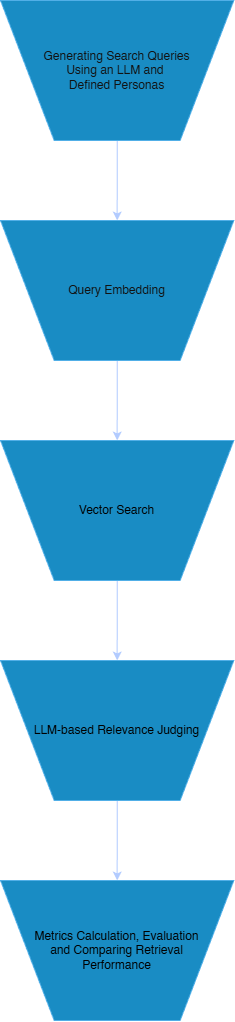
\includegraphics[width=0.4\linewidth]{pipeline.png}
    \Description{Vertical flowchart describing the general pipeline for both phases, showing query generation, judgment system, and metrics.}
    \caption{Vertical flowchart describing the general pipeline for both phases}
    \label{fig:hybrid-search-methodology}
\end{figure}

\subsection{Phase 1: Selecting the Best Dense Vector Model}
\label{subsec:phase1-dense-model-selection}

This phase evaluates seven state-of-the-art embedding models to identify the most effective dense vector representation for our pharmaceutical domain.

\subsubsection{Evaluated Models and Rationale}
\label{subsubsec:evaluated-models}

\begin{enumerate}
    \item \textbf{SBERT (MiniLM-L6-v2)}: A lightweight Sentence-BERT model optimized for semantic similarity tasks. Provides a strong baseline with efficient inference.

    \item \textbf{Bio\_ClinicalBERT}: A BERT model fine-tuned on clinical notes from MIMIC-III. Specifically designed for clinical text understanding, making it highly relevant for pharmaceutical documents.


    \item \textbf{PubMedBERT (NeuML)}: A BERT model pre-trained from scratch on PubMed abstracts and full-text articles. Domain-specific to biomedical literature.

    \item \textbf{SapBERT (PubMedBERT version)}: Specialized for biomedical entity linking, trained with self-alignment contrastive learning on UMLS concepts.

    \item \textbf{BGE Base (BAAI/bge-base-en-v1.5)}: A general-purpose embedding model optimized for retrieval tasks, supporting instructions and asymmetric search.

    \item \textbf{BioBERT Sentence (NLI/STS)}: A BioBERT model fine-tuned on multiple Natural Language Inference and Semantic Textual Similarity datasets, enhancing its understanding of biomedical text relationships.
\end{enumerate}

\subsubsection{Implementation Details}
\label{subsubsec:implementation-details}

The evaluation pipeline, implemented in Python, follows these steps:

\begin{enumerate}
    \item \textbf{Document Processing}: Each drug document is converted to a searchable text format combining brand name, generic name, purpose, indications and usage, active ingredients, and truncated warnings.

    \item \textbf{Vector Generation}: Models are loaded with GPU optimization where available, with batch processing (batch size 128-512 depending on model) and memory management to handle  VRAM constraints of loading so many models at the same time.

    \item \textbf{Solr Indexing}: Vectors are indexed in Apache Solr using the HNSW algorithm for efficient approximate nearest neighbor search with the following configuration:
          \begin{itemize}
              \item \texttt{efConstruction}: 200
              \item \texttt{M}: 16
              \item Distance function: Euclidean
          \end{itemize}

    \item \textbf{Search Execution}: For each query, the top $K=20$ documents are retrieved using ANN search.
\end{enumerate}

\subsubsection{Results and Analysis}
\label{subsubsec:phase1-results}

\begin{table}[htbp]
    \centering
    \caption{Performance comparison of dense vector models. Values show mean ± standard deviation across 20 queries.}
    \label{tab:dense-model-results}
    \begin{adjustbox}{width=\columnwidth}
        \begin{tabular}{lcccc}
            \hline
            \textbf{Model}    & \textbf{P@5}      & \textbf{P@10}     & \textbf{P@20}     & \textbf{MAP}      \\
            \hline
            SBERT             & 0.920 $\pm$ 0.214 & 0.860 $\pm$ 0.180 & 0.895 $\pm$ 0.152 & 0.198 $\pm$ 0.071 \\
            Bio\_ClinicalBERT & 0.770 $\pm$ 0.312 & 0.730 $\pm$ 0.217 & 0.733 $\pm$ 0.204 & 0.137 $\pm$ 0.062 \\
            PubMedBERT        & 0.940 $\pm$ 0.180 & 0.950 $\pm$ 0.153 & 0.935 $\pm$ 0.125 & 0.214 $\pm$ 0.059 \\
            SAPBERT\_PubMed   & 0.920 $\pm$ 0.147 & 0.845 $\pm$ 0.216 & 0.893 $\pm$ 0.158 & 0.193 $\pm$ 0.064 \\
            BGE               & 0.970 $\pm$ 0.071 & 0.940 $\pm$ 0.097 & 0.925 $\pm$ 0.070 & 0.209 $\pm$ 0.046 \\
            BioBERT\_Sentence & 0.900 $\pm$ 0.195 & 0.890 $\pm$ 0.170 & 0.902 $\pm$ 0.121 & 0.197 $\pm$ 0.054 \\
            \hline
        \end{tabular}
    \end{adjustbox}
\end{table}

\begin{figure}[htbp]
    \centering
    
\includegraphics[width=0.85\linewidth]{precision_recall_curve_11pt_avg_only.png}
    \Description{11-point interpolated precision-recall curve comparing multiple dense vector models. PubMedBERT consistently achieves higher precision across all recall levels.}
    \caption{Precision–Recall curve (11-point averaged)}
    \label{fig:pr_curve_11pt_dense}
\end{figure}


% PLACEHOLDER FOR PR CURVE COMMENT
\textbf{Precision-Recall Curve Analysis}: The 11-point interpolated precision-recall curves reveal that PubMedBert achieves the highest area under the curve, indicating superior retrieval performance across all recall levels. The curve shows particularly strong precision at lower recall levels (0.0-0.4), which is critical for user-facing search systems where only the top results are examined.

Based on the evaluation metrics, \textbf{PubMedBERT (NeuML)} was selected as the best-performing dense model for Phase 2, demonstrating superior performance in both early precision (P@5) and overall retrieval effectiveness (MAP).

\subsection{Phase 2: Tuning Hybrid Search Weight \texorpdfstring{$\alpha$}{alpha}}
\label{subsec:phase2-hybrid-tuning}

With PubMedBERT identified as the optimal dense model, this phase determines the best weighting parameter \texorpdfstring{$\alpha$}{alpha} for hybrid search combining dense PubMedBERT vectors with sparse BM25 retrieval.

\subsubsection{Hybrid Search Configuration}
\label{subsubsec:hybrid-configuration}

The hybrid search employs Reciprocal Rank Fusion (RRF) with the scoring function:

\[
    \text{score}(d) = \alpha \cdot \text{RRF}_{\text{vector}}(d) + (1 - \alpha) \cdot \text{RRF}_{\text{BM25}}(d)
\]

where $\text{RRF}(d) = \frac{1}{k + \text{rank}(d)}$ with $k = 20$.

The choice of $k=20$ reflects our focus on top results: we typically care about the top 5-10 results for user-facing drug label search, with a maximum consideration of 50 results for comprehensive retrieval.

\subsubsection{BM25 as Sparse Retrieval}
\label{subsubsec:bm25-rationale}

BM25 was selected for sparse retrieval due to:
\begin{itemize}
    \item \textbf{Superiority over TF-IDF}: BM25 addresses TF-IDF's limitations in term frequency saturation and document length normalization.
    \item \textbf{Proven Effectiveness}: Extensive research demonstrates BM25's strong performance in information retrieval tasks.
    \item \textbf{Term-Based Matching}: Provides complementary signals to semantic vector search, capturing exact term matches and phrase importance.
\end{itemize}

The BM25 search uses the same document text representation as vector models, indexed in Solr with standard text analysis (lowercasing, stemming, stopword removal).

\subsubsection{Alpha Parameter Sweep}
\label{subsubsec:alpha-sweep}

We evaluated $\alpha$ values from 0.30 to 0.70 in 0.10 increments:
\[
    \alpha \in \{0.30, 0.40, 0.50, 0.60, 0.70\}
\]

This range tests configurations from BM25-dominated ($\alpha=0.30$) to vector-dominated ($\alpha=0.70$) hybrid search, with equal weighting at $\alpha=0.50$.

\subsubsection{Results and Optimal $\alpha$ Selection}
\label{subsubsec:phase2-results}

\begin{table}[htbp]
    \centering
    \caption{Hybrid search performance across $\alpha$ values. PubMedBERT + BM25 with RRF ($k=20$).}
    \label{tab:hybrid-alpha-results}
    \begin{adjustbox}{width=\columnwidth}
        \begin{tabular}{lcccc}
            \hline
            \textbf{$\alpha$} & \textbf{P@5}      & \textbf{P@10}     & \textbf{P@20}     & \textbf{MAP}      \\
            \hline
            0.30              & 0.950 $\pm$ 0.124 & 0.975 $\pm$ 0.062 & 0.933 $\pm$ 0.112 & 0.508 $\pm$ 0.093 \\
            0.40              & 0.950 $\pm$ 0.124 & 0.975 $\pm$ 0.062 & 0.970 $\pm$ 0.083 & 0.530 $\pm$ 0.084 \\
            0.50              & 0.960 $\pm$ 0.102 & 0.970 $\pm$ 0.064 & 0.975 $\pm$ 0.040 & 0.533 $\pm$ 0.049 \\
            0.60              & 0.980 $\pm$ 0.060 & 0.980 $\pm$ 0.051 & 0.965 $\pm$ 0.069 & 0.529 $\pm$ 0.053 \\
            0.70              & 0.980 $\pm$ 0.060 & 0.980 $\pm$ 0.051 & 0.950 $\pm$ 0.105 & 0.522 $\pm$ 0.064 \\
            \hline
        \end{tabular}
    \end{adjustbox}
\end{table}


Table~\ref{tab:hybrid-alpha-results} demonstrates the substantial performance gain achieved by hybridizing PubMedBERT with BM25, with MAP scores (0.508-0.533) more than doubling those of the best dense model alone (0.214). This confirms the complementary nature of semantic and keyword-based retrieval. The results show a clear performance peak at $\alpha=0.50$, which achieves the highest P@20 (0.975) and MAP (0.533). While $\alpha=0.60$ and $\alpha=0.70$ yield marginally higher P@5 and P@10 (0.980), they exhibit declining performance at deeper recall (P@20) and overall effectiveness (MAP). This suggests that over-weighting the dense vector component, while beneficial for top-ranked precision, may compromise the diversity and completeness of results. The balanced weighting ($\alpha=0.50$) provides the optimal trade-off, maximizing both early precision and comprehensive recall. Notably, all hybrid configurations significantly outperform individual methods, with remarkably low standard deviations indicating consistent high performance across diverse queries.




\begin{figure}[htbp]
    \centering
    
\includegraphics[width=0.85\linewidth]{precision_recall_curve_hybrid_alpha_compare.png}
    \Description{Precision-recall curve comparing different alpha values for hybrid search. An alpha of 0.50 performs best across most recall levels.}
    \caption{Precision–Recall curve (11-point averaged)}
    \label{fig:pr_curve_11pt_hybrid}
\end{figure}



\textbf{Precision-Recall Curve Analysis}: The hybrid P-R curves show that intermediate $\alpha$ values (0.40-0.60) achieve the highest area under the curve, with $\alpha=0.50$ maintaining strong precision across the entire recall spectrum. The curves confirm that hybrid search dramatically outperforms either method in isolation, particularly at medium to high recall levels where pure vector search typically degrades. Note that for every alpha tested results were extremely good, because of the precision of both the ANN selected and the BM25.

\subsection{Hybrid Model Findings}
\label{subsec:hybrid-model-findings}

This two-phase investigation successfully identified an optimal hybrid search configuration for pharmaceutical document retrieval. Phase 1 evaluated six dense embedding models, with PubMedBERT emerging as the most effective single model due to its superior MAP (0.214) and balanced precision across ranking depths. Phase 2 demonstrated that hybridizing PubMedBERT with BM25 using Reciprocal Rank Fusion yields dramatic performance improvements, with MAP scores increasing by approximately 150\% across all tested $\alpha$ values. The optimal configuration was achieved with equal weighting ($\alpha=0.50$), producing a system with P@5=0.960, P@10=0.970, P@20=0.975, and MAP=0.533. This configuration optimally balances the semantic understanding of PubMedBERT with the exact term matching of BM25, creating a robust retrieval system capable of handling diverse pharmaceutical queries with high precision and recall. The final hybrid system substantially outperforms either approach in isolation, validating the hybrid search paradigm for this specialized domain.



\section{Frontend Development}
\label{sec:frontend-development}

Following the identification of the optimal hybrid search configuration (PubMedBERT with BM25 at $\alpha=0.50$), we developed a comprehensive web-based frontend to showcase the system's capabilities and provide an intuitive interface for end-users. The frontend serves dual purposes: it functions as a production-ready search interface for medical professionals while simultaneously demonstrating the effectiveness of our retrieval system through transparent result presentation.

\begin{figure}[htbp]
    \centering
    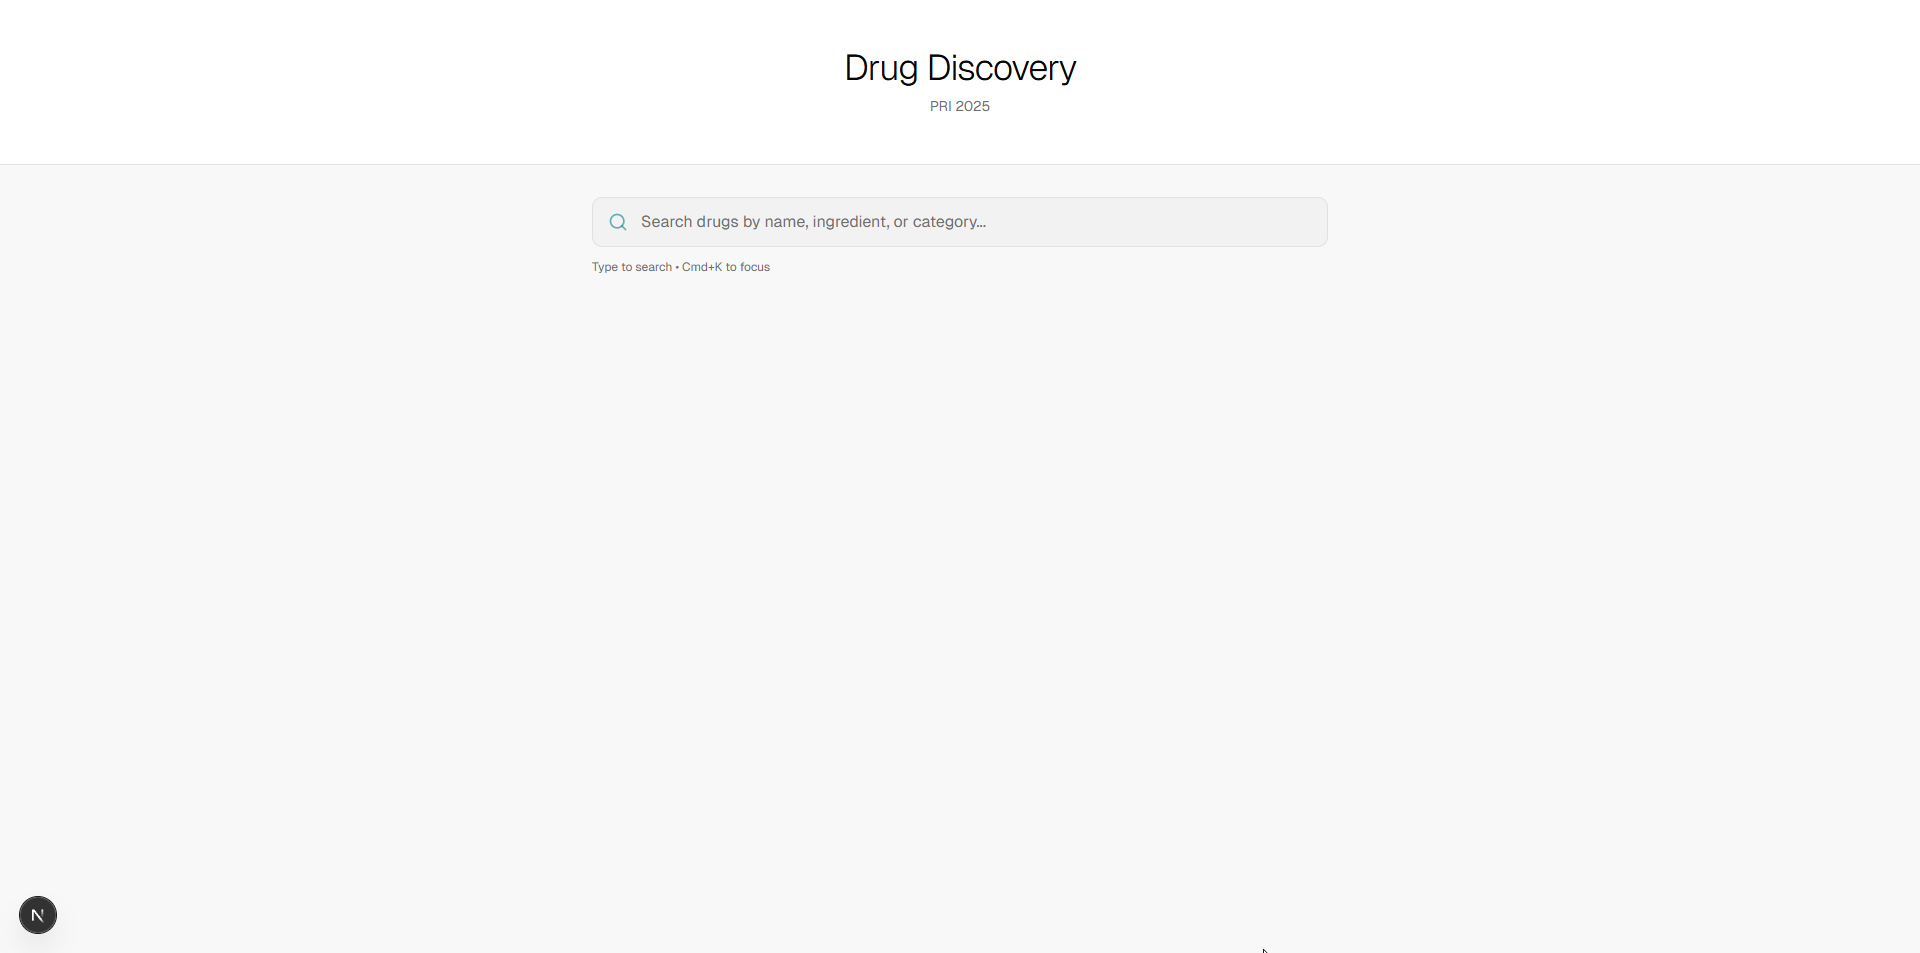
\includegraphics[width=0.85\linewidth]{frontend1.png}
    \Description{Screenshot of the search interface in its idle state, showing a clean search bar and navigation elements.}
    \caption{Idle Interface}
    \label{fig:frontend_idle}
\end{figure}


\subsection{Query Rewriting and Smart Filtering}

To improve search precision, the frontend implements a sophisticated client-side query rewriting and smart filtering system. Its primary goal is to interpret user input correctly by distinguishing between free-text search terms and structured filters. This is especially important because an uninformed user might enter terms that are ambiguous. For example, a search for ``oral'' intending to find oral pills could return results marked ``not for oral use,'' causing confusion. Smart filtering helps prevent such mismatches by mapping user intent to structured fields, which are then sent as Solr filter queries (fq) to refine search results. For instance, if a user types ``oral,'' the system converts this into the Solr filter query \texttt{fq=route:oral}.


\paragraph{Discovery of Key Filters}
Through analysis of the database and running scripts to examine which categorical fields were worth filtering, three primary categories were identified:
\begin{itemize}
    \item \textbf{Route of administration} (e.g., oral, intravenous)
    \item \textbf{Therapeutic category} (e.g., Analgesics, Antivirals)
    \item \textbf{Product type} (e.g., HUMAN OTC DRUG, HUMAN PRESCRIPTION DRUG)
\end{itemize}

\paragraph{Handling Aliases and Variations}
To improve matching accuracy, several strategies were implemented:

\begin{itemize}
    \item \textbf{Singular and Plural Forms:} Many therapeutic categories are plural (e.g., ``Analgesics''), so singular versions were added to the lookup to match queries like ``analgesic.''

    \item \textbf{User-Friendly Aliases for Product Types:} Product type names are often long and unintuitive (e.g., ``HUMAN OTC DRUG''). To accommodate natural language queries, aliases were added:
          \begin{itemize}
              \item ``HUMAN OTC DRUG'' $\to$ [``otc'', ``shelf'', ``over the counter'', ``generic'', ``generical'']
              \item ``HUMAN PRESCRIPTION DRUG'' $\to$ [``prescription'', ``prescribed'', ``rx'', ``script'']
          \end{itemize}

    \item \textbf{Synonyms for Routes and Therapeutic Categories:} Common synonyms and related terms were included to capture user intent. Examples include:
          \begin{itemize}
              \item Routes: ``mouth'' $\to$ ``oral'', ``nose'' $\to$ ``nasal'', ``iv'' $\to$ ``intravenous'', ``im'' $\to$ ``intramuscular''
              \item Therapeutic categories: ``anxiety'' $\to$ ``Anxiolytics'', ``virus'' $\to$ ``Antivirals'', ``pain'' $\to$ ``Analgesics''
          \end{itemize}
\end{itemize}

\paragraph{Implementation}
The \texttt{extractFilterFromQuery} function scans user input for these canonical terms, singular/plural variants, and aliases. When a match is found:
\begin{itemize}
    \item The matched term is removed from the query string.
    \item A structured filter object is created containing the canonical category, the matched alias, and a display value.
    \item The user sees the parsed filters as ``chips'' or tags in the interface, providing immediate feedback that the system correctly interpreted their intent.
\end{itemize}

This multi-layered approach ensures that user searches are both intuitive and precise, minimizing irrelevant results and improving the overall user experience in the drug discovery application.

\begin{figure}[htbp]
    \centering
    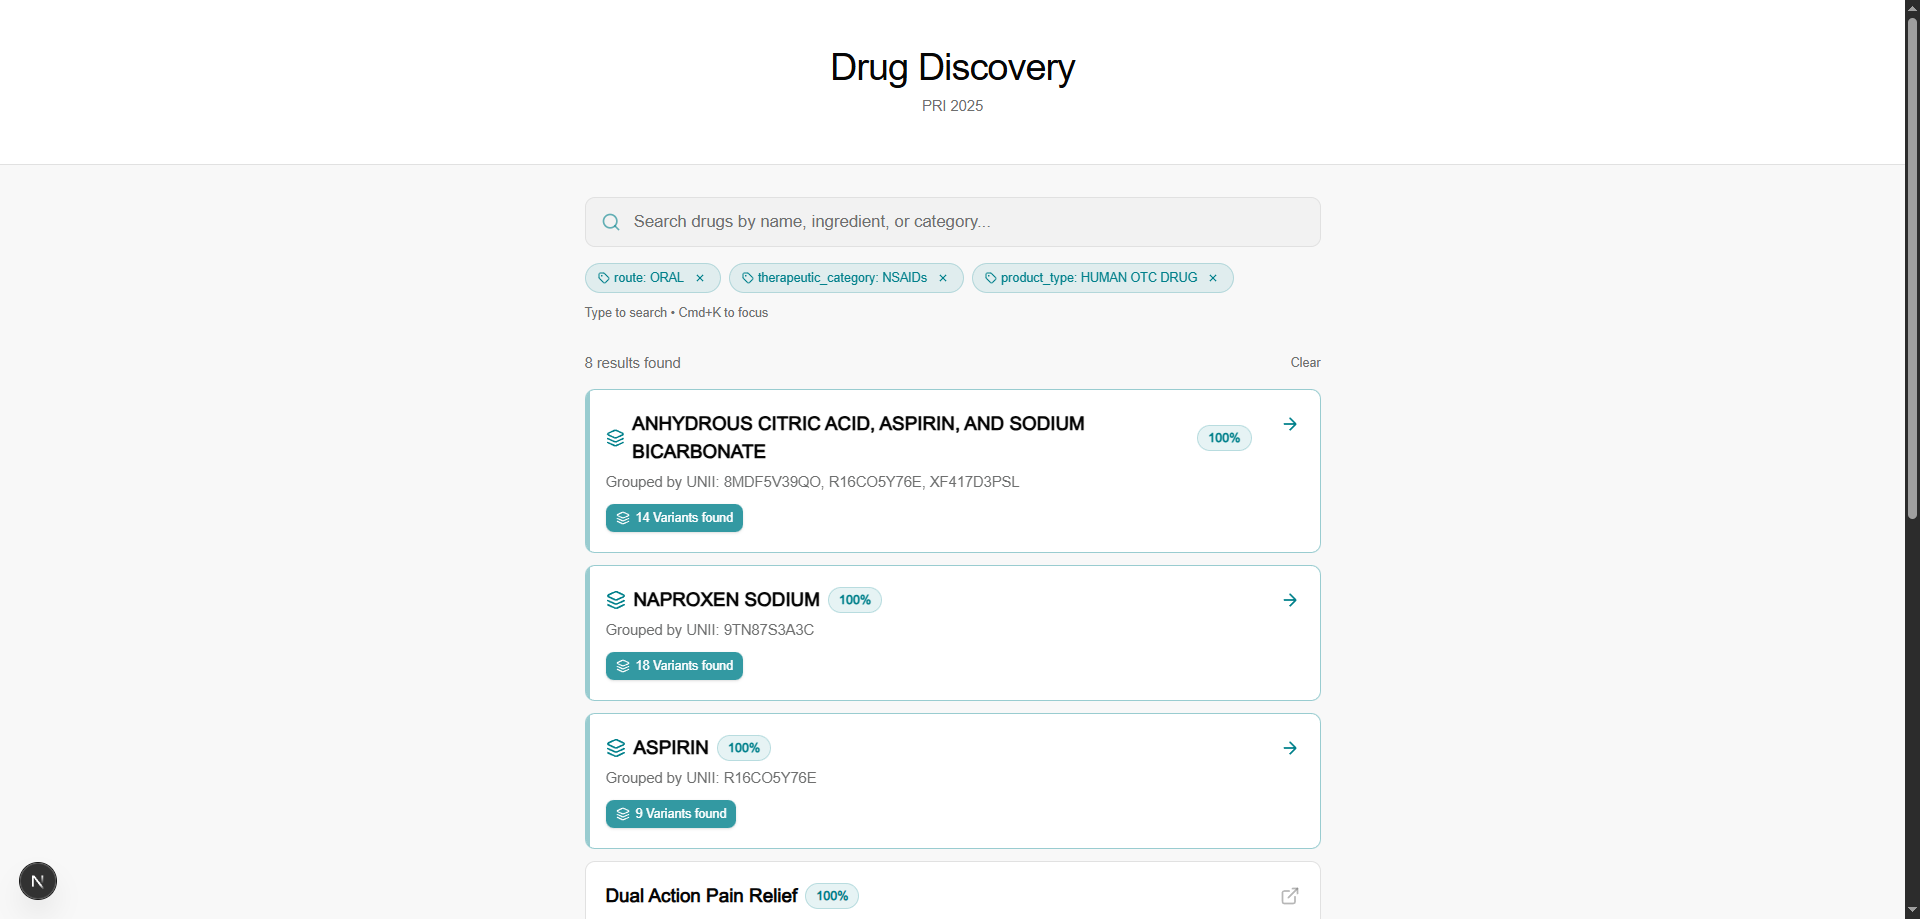
\includegraphics[width=0.85\linewidth]{frontend5.png}
    \Description{Screenshot showing query results where 'oral nsaid otc' is automatically converted into structured filters for route, category, and product type.}
    \caption{Example query results showcasing Query Rewriting and Smart Filtering (typing "oral nsaid otc" is rewritten to the following fq solr filters)}
    \label{fig:frontend_query_rewrite}
\end{figure}

\subsection{Results Clustering}

Medical databases often contain numerous entries for the same drug active ingredient (e.g., hundreds of brands of Ibuprofen). To prevent result flooding and improve navigability, the system implements result clustering based on the Unique Ingredient Identifier (UNII).

\begin{itemize}
    \item \textbf{Backend Grouping:} The backend groups raw Solr results by their UNII set. If multiple products share the exact same active ingredients, they are collapsed into a single "Cluster" object.

    \item \textbf{Scoring:} The relevance score of a cluster is determined by the highest-scoring individual variant within it, ensuring that the most relevant grouping appears at the top.

    \item \textbf{Frontend Representation:} In the user interface, clusters are visually distinct from single drug results. They display a badge indicating the number of variants (e.g., "12 Variants found").

    \item \textbf{Interaction:} Clicking on a cluster triggers a "drill-down" view (\texttt{activeCluster} state), replacing the main list with the specific variants contained within that group. This allows users to first find the correct drug ingredient and then select the specific manufacturer or dosage form.
\end{itemize}

\begin{figure}[htbp]
    \centering
    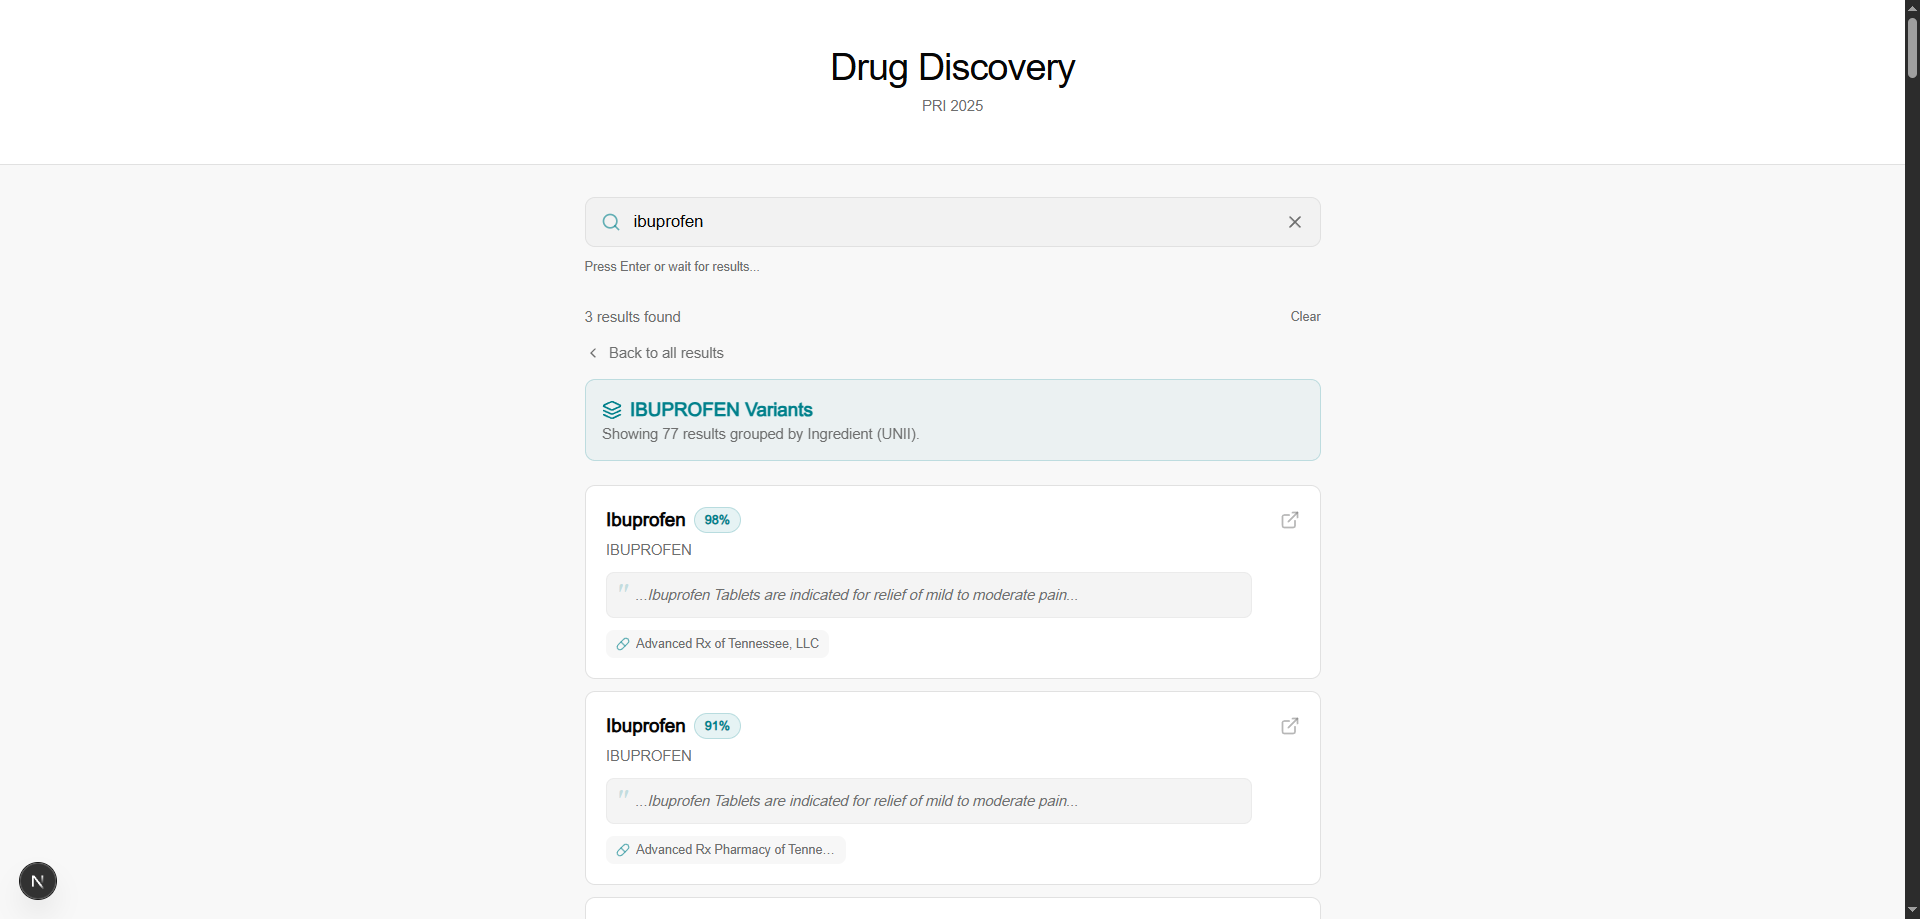
\includegraphics[width=0.85\linewidth]{frontend3.png}
    \Description{Screenshot of search results grouped by cluster, showing multiple variants of a drug under a single ingredient heading.}
    \caption{Example of search results inside a cluster}
    \label{fig:frontend_cluster}
\end{figure}

\subsection{Semantic Snippet Generation}

To explain \textit{why} a specific result was retrieved—especially for vector-based semantic searches where keywords might not visually match—the system generates context-aware snippets. (e.g., displaying "...relief of mild to moderate pain..." for a search query of "headache").

\begin{itemize}
    \item \textbf{Vector-Based Highlighting:} Standard keyword highlighting fails when the match is semantic (e.g., query "pain" matches text "analgesic"). Instead, the backend uses the SBERT model to compare the user's query vector against individual sentences within the drug's description fields (Purpose, Indications).

    \item \textbf{Batch Processing:} To maintain performance, snippet generation is batched. The backend collects candidate sentences from the top retrieved documents and encodes them in a single inference pass.

    \item \textbf{Thresholding:} Only sentences with a high cosine similarity score ($>0.4$) to the query are returned as snippets. Because of this, some search results don't have semantic snippets at all.

\end{itemize}

\begin{figure}[htbp]
    \centering
    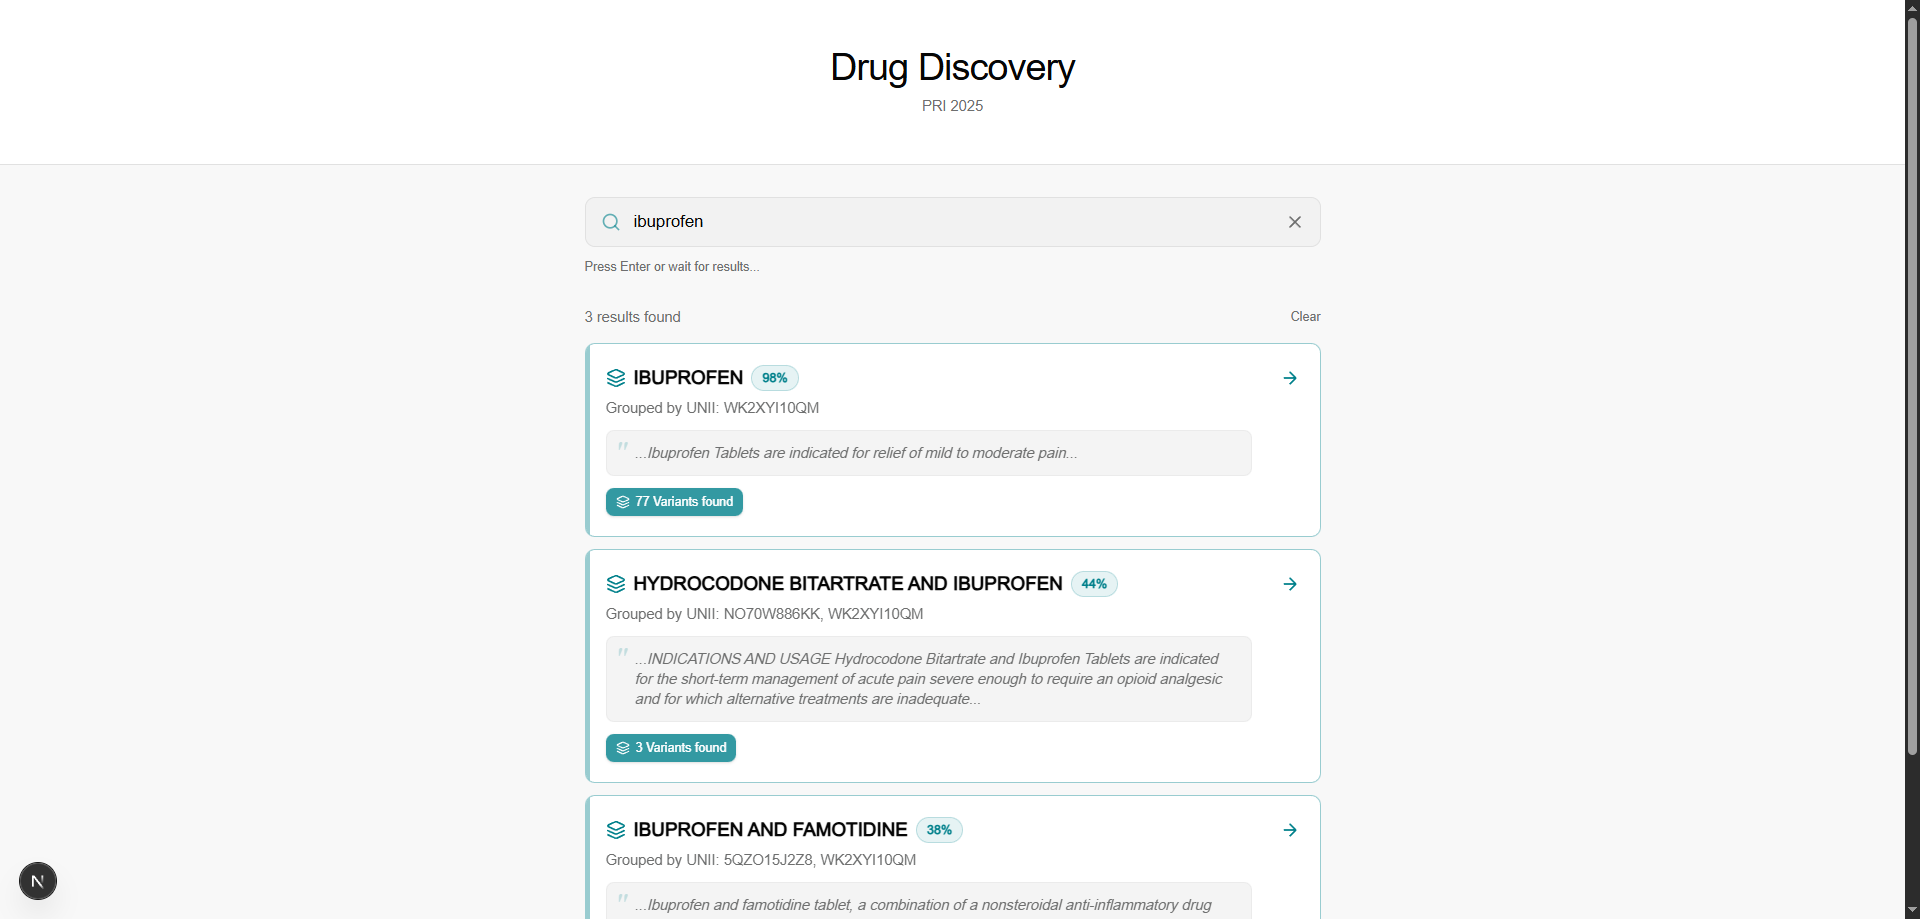
\includegraphics[width=0.85\linewidth]{frontend2.png}
    \Description{Screenshot showing search results with semantic snippets highlighted, explaining why the result matched the query.}
    \caption{Example of several snippet generations}
    \label{fig:frontend_snippet}
\end{figure}


\subsection{Relevance Feedback: More Like This}

To further enhance search precision, we implemented an explicit relevance feedback mechanism. When viewing a drug's details, users can request "Similar Drugs". This triggers a Solr MoreLikeThis (MLT) query using the current document's key fields (Purpose, Indications, Active Ingredients) as the seed. This feature allows users to pivot from a single relevant result to a broader set of related medications without manually refining their query keywords, effectively satisfying the project's suggestion for relevance feedback.


\subsection{External Data Linking: PubChem Integration}

To fulfill the objective of enriching the system with external data sources, we integrated dynamic linking to the PubChem database. Rather than statically importing massive image datasets, we implemented a real-time integration using the PubChem PUG REST API. When a user views a drug's details, the frontend dynamically fetches the 2D chemical structure image using the drug's \texttt{generic\_name} as the key. This approach significantly enhances the user experience by providing immediate visual context for chemical compounds without the overhead of local storage.


\begin{figure}[htbp]
    \centering
    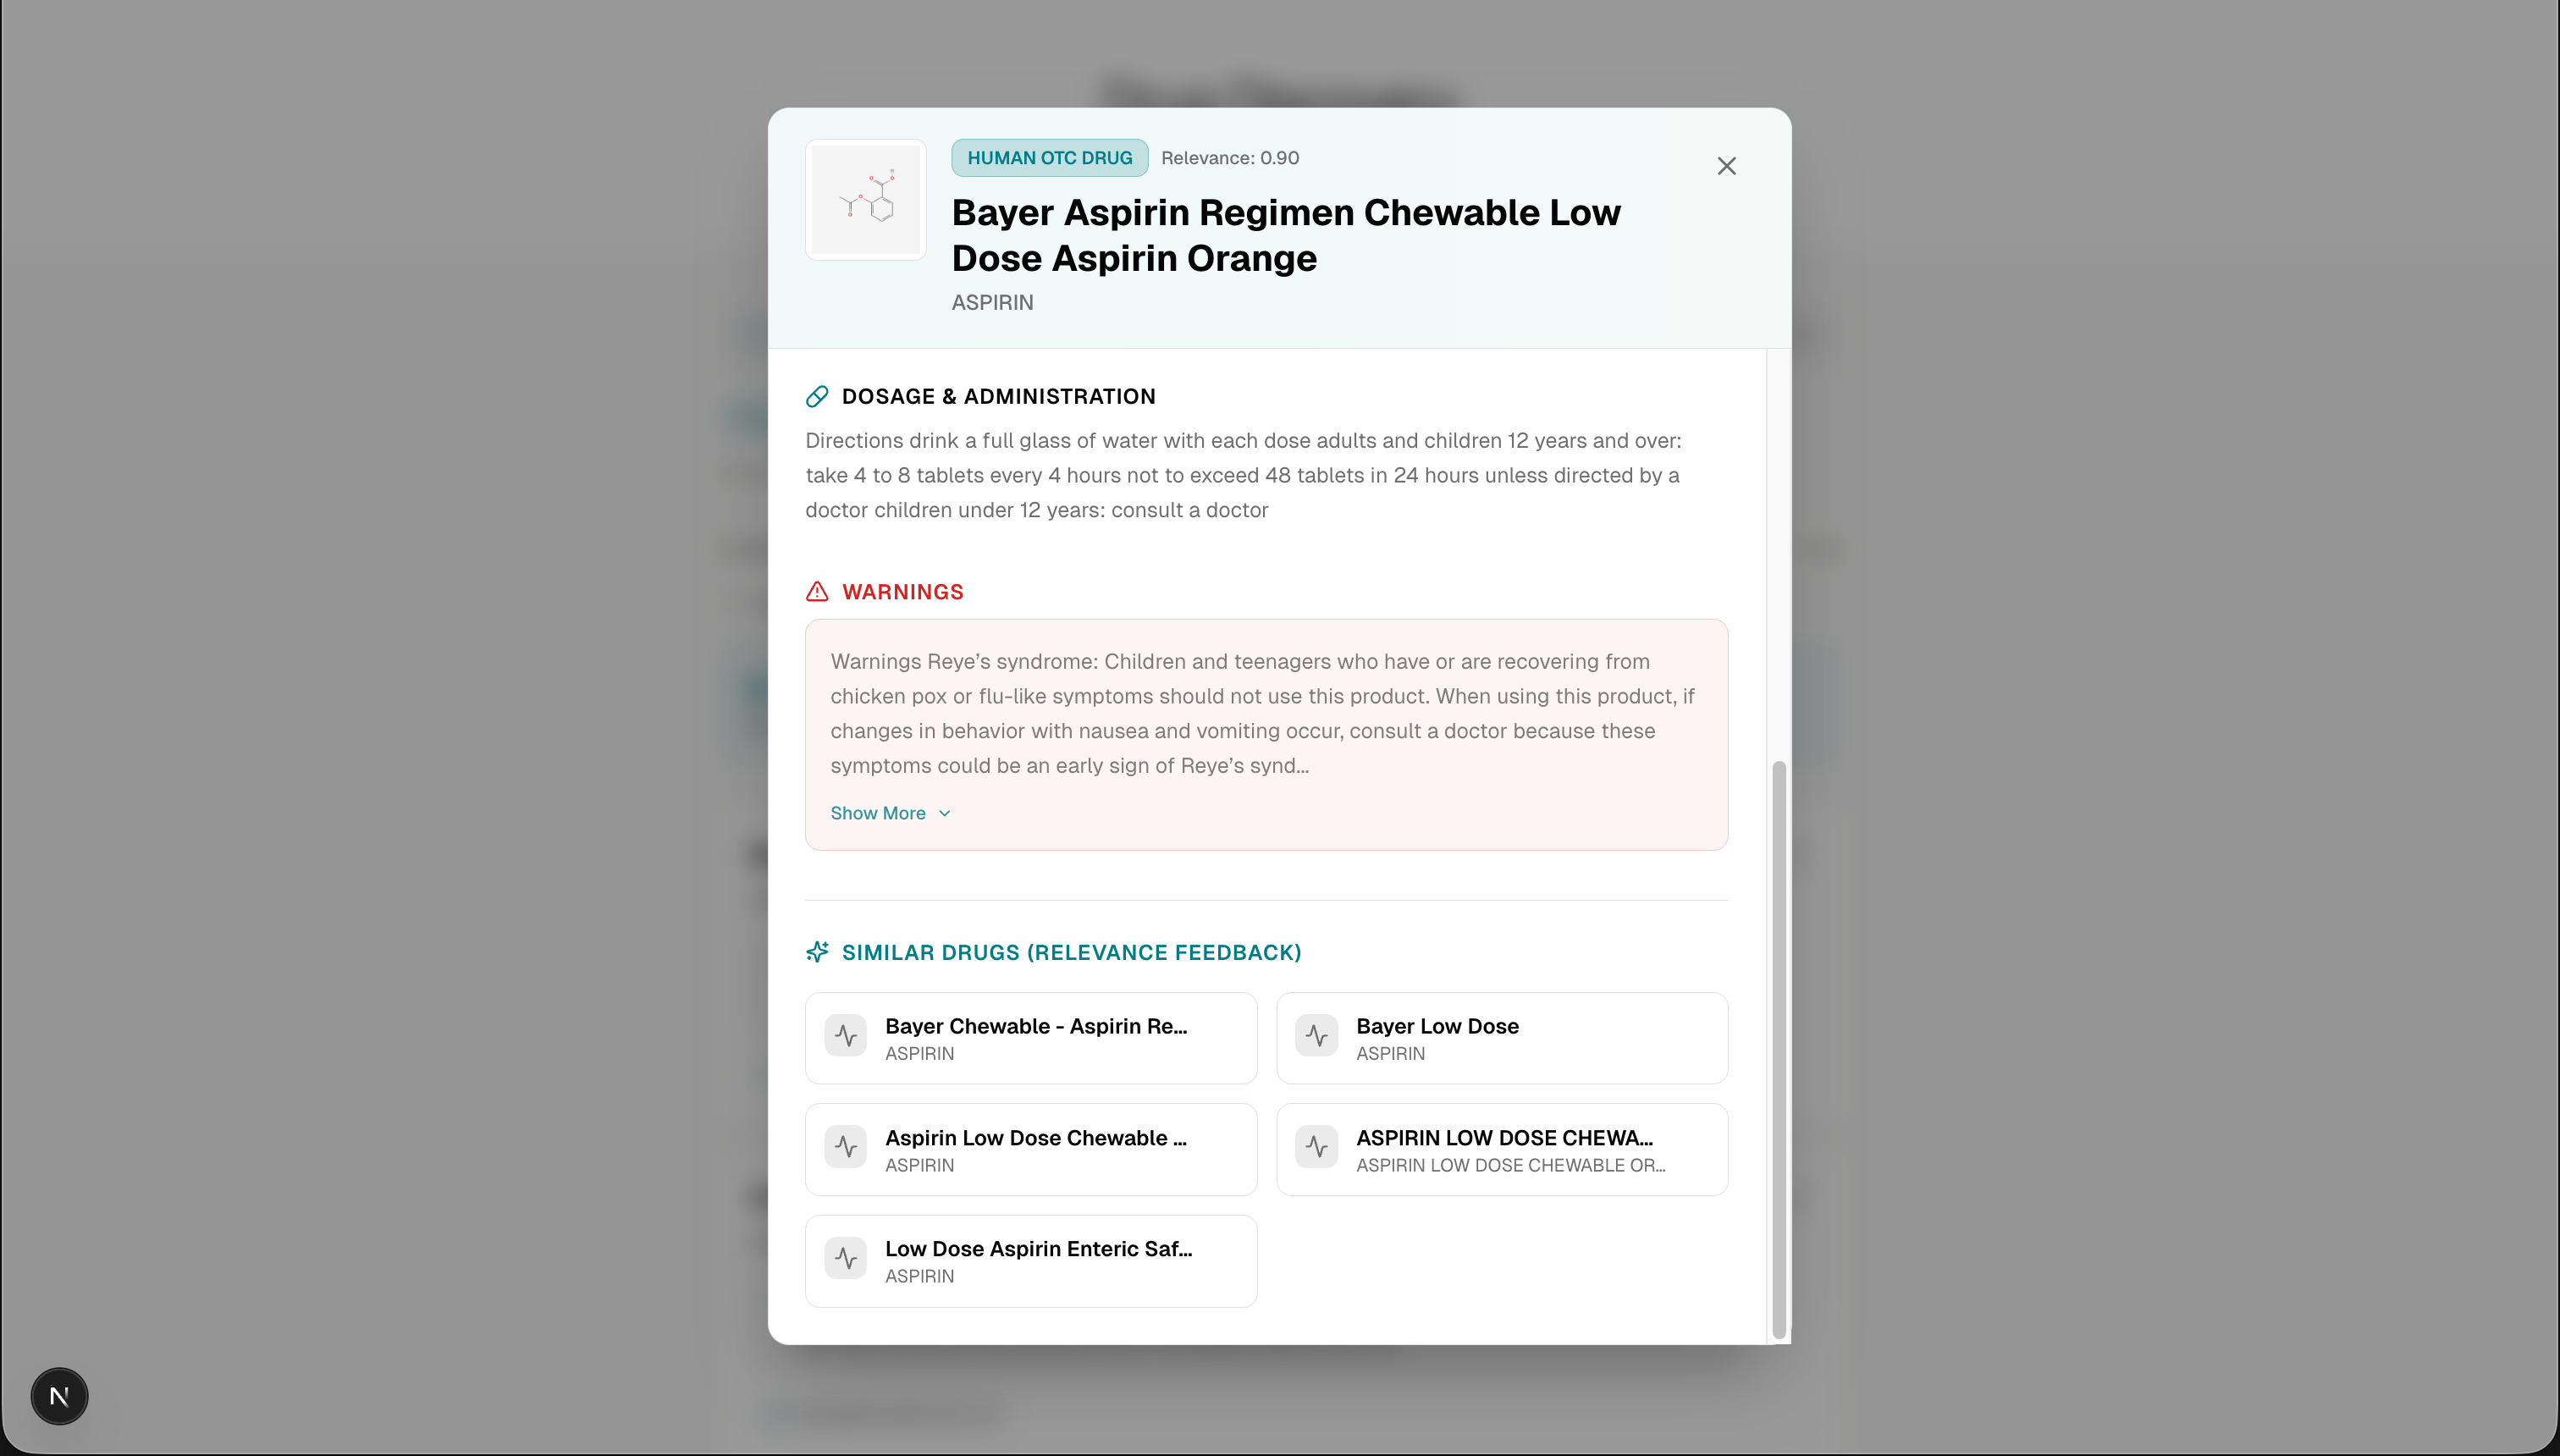
\includegraphics[width=1\linewidth]{frontend6.png}
    \Description{Screenshot of the detail modal view, displaying comprehensive structure data for a specific drug.}
    \caption{Showcase of DetailModel}
    \label{fig:frontend_detail_modal}
\end{figure}

\subsection{User Interface Components}

The application is composed of three main modular components to eansure maintainability and responsiveness:

\begin{itemize}
    \item \textbf{SearchBar:} Handles the real-time parsing of input and display of active filters.

    \item \textbf{SearchResults:} Renders the list of drugs and clusters, managing the transition between the main list view and the cluster drill-down view.

    \item \textbf{DetailModal:} Provides a comprehensive view of a selected drug's structured data (active ingredients, dosage, warnings, etc.) without navigating away from the search context.
\end{itemize}


% =============================
% Part 4: Conclusion
% =============================
\section{Conclusion}
\label{sec:conclusion}

This project successfully developed a comprehensive drug information retrieval system, evolving from a raw data pipeline to a sophisticated hybrid search application.

The development began with establishing a robust data foundation by ingesting and characterizing datasets from OpenFDA and DrugBank. We defined a clear conceptual model centered on the "Drug" entity and implemented a reproducible ETL pipeline to clean and structure this diverse data.

Building on this foundation, we focused on core retrieval capabilities using Apache Solr. We implemented and evaluated multiple retrieval configurations, establishing a strong baseline using standard text analysis techniques. Our manual evaluation framework allowed us to quantify the performance of different field weighting strategies.

Subsequently, we significantly advanced the state of the art of our system by implementing a Hybrid Search architecture. Our extensive evaluation of dense vector models identified \textbf{PubMedBERT (NeuML)} as the superior embedding model for this domain. By combining this semantic signal with BM25 keyword matching using Reciprocal Rank Fusion (RRF), we achieved a dramatic performance improvement, with the optimal configuration ($\alpha=0.5$) doubling the Mean Average Precision (MAP) compared to vector-only search.

Finally, we wrapped these backend advances in a modern, user-centric frontend. Features like \textbf{Smart Filtering}, \textbf{Result Clustering}, \textbf{Semantic Snippets}, and \textbf{Visual Chemical Structures} (via PubChem) directly address real-world user needs for precision and explainability. The system now stands as a complete, end-to-end solution for pharmaceutical information retrieval, offering both high-accuracy search and an intuitive, feature-rich discovery experience. Future work could explore personalized ranking based on user history and expanding the knowledge graph with drug-interaction data.


\clearpage

\bibliographystyle{ACM-Reference-Format}
\bibliography{bib/references}

\appendix
\appendix
\section*{Appendix}
\section{Analysis Configuration}
\label{appendix:analysis}

The analysis configuration for \texttt{text\_general} was applied via analysis.json. The field type was modified to include a PorterStemFilterFactory for stemming:

\begin{minted}[fontsize=\scriptsize]{json}
{
  "replace-field-type": {
    "name": "text_general",
    "class": "solr.TextField",
    "positionIncrementGap": "100",
    "analyzer": {
      "tokenizer": {
        "class": "solr.StandardTokenizerFactory"
      },
      "filters": [
        { "class": "solr.LowerCaseFilterFactory" },
        { "class": "solr.PorterStemFilterFactory" }
      ]
    }
  }
}
\end{minted}

\section{Solr Add-Field Schema}
\label{appendix:addfield}

The full JSON add-field request used to define the Solr schema is shown below:

\begin{minted}[fontsize=\scriptsize]{json}
{
  "add-field": [
    {"name":"version","type":"pint","stored":true,"indexed":true,"multiValued":false},
    {"name":"effective_time","type":"pdate","stored":true,"indexed":true,"multiValued":false},
    {"name":"product_ndc","type":"string","stored":true,"indexed":true,"multiValued":true},
    {"name":"primary_ndc","type":"string","stored":true,"indexed":true,"multiValued":true},
    {"name":"package_ndc","type":"string","stored":true,"indexed":true,"multiValued":true},
    {"name":"drug_id","type":"string","stored":true,"indexed":true,"multiValued":false},
    {"name":"set_id","type":"string","stored":true,"indexed":true,"multiValued":false},
    {"name":"therapeutic_category","type":"text_general","stored":true,"indexed":true,
     "multiValued":true},
    {"name":"brand_name","type":"text_general","stored":true,"indexed":true,"multiValued":false},
    {"name":"generic_name","type":"text_general","stored":true,"indexed":true,"multiValued":false},
    {"name":"manufacturer","type":"text_general","stored":true,"indexed":true,"multiValued":false},
    {"name":"route","type":"text_general","stored":true,"indexed":true,"multiValued":true},
    {"name":"substance_name","type":"text_general","stored":true,"indexed":true,"multiValued":true},
    {"name":"product_type","type":"text_general","stored":true,"indexed":true,"multiValued":false},
    {"name":"unii","type":"string","stored":true,"indexed":true,"multiValued":true},
    {"name":"indications_and_usage","type":"text_general","stored":true,"indexed":true,"multiValued":false},
    {"name":"dosage_and_administration","type":"text_general","stored":true,"indexed":true,"multiValued":false},
    {"name":"purpose","type":"text_general","stored":true,"indexed":true,"multiValued":false},
    {"name":"warnings","type":"text_general","stored":true,"indexed":true,"multiValued":false},
    {"name":"active_ingredients","type":"text_general","stored":true,"indexed":true,"multiValued":false},
    {"name":"inactive_ingredients","type":"text_general","stored":true,"indexed":true,"multiValued":false},
    {"name":"storage_and_handling","type":"text_general","stored":true,"indexed":true,"multiValued":false}
  ]
}
\end{minted}

\section{Copy Fields Definition}
\label{appendix:copyfields}

The following copy-field definitions were applied via \texttt{copy\_fields.json} to consolidate content from multiple fields into \texttt{text\_all}:

\begin{minted}[fontsize=\scriptsize]{json}
{
  "add-copy-field": [
    { "source": "brand_name", "dest": "text_all" },
    { "source": "generic_name", "dest": "text_all" },
    { "source": "therapeutic_category", "dest": "text_all" },
    { "source": "indications_and_usage", "dest": "text_all" },
    { "source": "dosage_and_administration", "dest": "text_all" },
    { "source": "purpose", "dest": "text_all" },
    { "source": "warnings", "dest": "text_all" },
    { "source": "active_ingredients", "dest": "text_all" }
  ]
}
\end{minted}
\section{Relevance Judgment Criteria}
\label{appendix:relevance-criteria}

The specific instruction prompt used for the manual/AI-assisted relevance evaluation (Section~\ref{sec:example-setup}) is defined as follows:

\begin{quote}
  \textit{Assign a binary relevance score of 1 (Relevant) or 0 (Irrelevant) to the provided document based on the following specific user need: A pregnant woman requires a safe, oral, over-the-counter (OTC) medication for fever or headache, with product information updated between 2023 and 2025.}

  \textit{To be marked Relevant (1), the document must satisfy all five conditions:}
  \begin{itemize}
    \item \textit{Explicitly indicates treatment for fever or headache.}
    \item \textit{Specifies an oral administration route (e.g., tablet, liquid).}
    \item \textit{Is classified as OTC.}
    \item \textit{Includes a date within the 2023-2025 range.}
    \item \textit{Does not strictly contraindicate use during pregnancy.}
  \end{itemize}
\end{quote}

\section{Hybrid Search Implementation}
\label{appendix:hybrid-code}

The core Reciprocal Rank Fusion (RRF) logic implemented in the backend API to combine PubMedBERT vectors and BM25 scores:

\begin{minted}[fontsize=\scriptsize]{python}
# RRF Logic: score = alpha * (1 / (k + rank)) + (1-alpha) * (1 / (k + rank))
def apply_rrf(docs, rank_weight):
    for rank, doc in enumerate(docs, 1):
        doc_id = str(doc.get('drug_id'))
        if not doc_id: continue
        
        # Calculate RRF component
        rr = 1 / (RRF_K + rank)
        score_contrib = rank_weight * rr
        
        fused_scores[doc_id] = fused_scores.get(doc_id, 0) + score_contrib

# Apply Vector Ranks (Alpha = 0.5)
apply_rrf(vector_docs, ALPHA)

# Apply BM25 Ranks (1 - Alpha = 0.5)
apply_rrf(bm25_docs, (1 - ALPHA))
\end{minted}

\end{document}
